% Options for packages loaded elsewhere
\PassOptionsToPackage{unicode}{hyperref}
\PassOptionsToPackage{hyphens}{url}
%
\documentclass[
]{article}
\usepackage{amsmath,amssymb}
\usepackage{iftex}
\ifPDFTeX
  \usepackage[T1]{fontenc}
  \usepackage[utf8]{inputenc}
  \usepackage{textcomp} % provide euro and other symbols
\else % if luatex or xetex
  \usepackage{unicode-math} % this also loads fontspec
  \defaultfontfeatures{Scale=MatchLowercase}
  \defaultfontfeatures[\rmfamily]{Ligatures=TeX,Scale=1}
\fi
\usepackage{lmodern}
\ifPDFTeX\else
  % xetex/luatex font selection
\fi
% Use upquote if available, for straight quotes in verbatim environments
\IfFileExists{upquote.sty}{\usepackage{upquote}}{}
\IfFileExists{microtype.sty}{% use microtype if available
  \usepackage[]{microtype}
  \UseMicrotypeSet[protrusion]{basicmath} % disable protrusion for tt fonts
}{}
\makeatletter
\@ifundefined{KOMAClassName}{% if non-KOMA class
  \IfFileExists{parskip.sty}{%
    \usepackage{parskip}
  }{% else
    \setlength{\parindent}{0pt}
    \setlength{\parskip}{6pt plus 2pt minus 1pt}}
}{% if KOMA class
  \KOMAoptions{parskip=half}}
\makeatother
\usepackage{xcolor}
\usepackage[margin=1in]{geometry}
\usepackage{longtable,booktabs,array}
\usepackage{calc} % for calculating minipage widths
% Correct order of tables after \paragraph or \subparagraph
\usepackage{etoolbox}
\makeatletter
\patchcmd\longtable{\par}{\if@noskipsec\mbox{}\fi\par}{}{}
\makeatother
% Allow footnotes in longtable head/foot
\IfFileExists{footnotehyper.sty}{\usepackage{footnotehyper}}{\usepackage{footnote}}
\makesavenoteenv{longtable}
\usepackage{graphicx}
\makeatletter
\def\maxwidth{\ifdim\Gin@nat@width>\linewidth\linewidth\else\Gin@nat@width\fi}
\def\maxheight{\ifdim\Gin@nat@height>\textheight\textheight\else\Gin@nat@height\fi}
\makeatother
% Scale images if necessary, so that they will not overflow the page
% margins by default, and it is still possible to overwrite the defaults
% using explicit options in \includegraphics[width, height, ...]{}
\setkeys{Gin}{width=\maxwidth,height=\maxheight,keepaspectratio}
% Set default figure placement to htbp
\makeatletter
\def\fps@figure{htbp}
\makeatother
\setlength{\emergencystretch}{3em} % prevent overfull lines
\providecommand{\tightlist}{%
  \setlength{\itemsep}{0pt}\setlength{\parskip}{0pt}}
\setcounter{secnumdepth}{5}
\ifLuaTeX
  \usepackage{selnolig}  % disable illegal ligatures
\fi
\usepackage[]{natbib}
\bibliographystyle{plainnat}
\usepackage{bookmark}
\IfFileExists{xurl.sty}{\usepackage{xurl}}{} % add URL line breaks if available
\urlstyle{same}
\hypersetup{
  pdftitle={CS448Notes},
  pdfauthor={Yash Mali},
  hidelinks,
  pdfcreator={LaTeX via pandoc}}

\title{CS448Notes}
\author{Yash Mali}
\date{}

\begin{document}
\maketitle

{
\setcounter{tocdepth}{2}
\tableofcontents
}
\section{CPSC 448 Notes}\label{cpsc-448-notes}

Directed studies on optimization in ML and advanced deep learning architectures.

\section{Gradient Descent Analysis}\label{gradient-descent-analysis}

\subsection{Gradient descent background}\label{gradient-descent-background}

Gradient descent is an iterative optimization algorithm that was first proposed in 1847 by Cauchy. The algorithm can be summarized as follows:

\[
w^t = w^{t-1} - \alpha_t \nabla f(w^t) \\
\text{  For t = 1, 2, 3 ...}
\]

Where we are trying to find a set of parameters \(w\) that minimize the function \(f\), also called the objective function. \(\nabla f\) is the gradient of \(f\) with respect to \(w\) and the subscript \(t\) is the iteration number.

The main idea is to move in the opposite direction of the steepest ascent of the function \(f\). How much you move during each iteration is controlled by two things. The first is the steepness of gradient which we cannot control after we have chosen the objective function. The second is the parameter \(\alpha_t\). It is also called th learning rate.

The time complexity of \textbf{each} iteration is only \(O(d)\) after computing the gradient. Where \(d\) is the number of parameters. We can stop if we have made very little progress, \(||f(w^t) - f(w^{t-1})||\) is very small.

Intuitively gradient descent can be thought of as standing on the top of a canyon while being blindfolded and using your leg to find the steepest slope downwards locally. Then, taking a small step in that direction and repeating the process until you reach the bottom. In this analogy the canyon can be thought of as modelled by a 3D objective function.

\subsection{Showing gradient descent reduces the objective function.}\label{showing-gradient-descent-reduces-the-objective-function.}

Let us assume that the objective function is Lipschitz continuous. Intuitively it means that a this function does not change in gradient arbitrarily fast. Formally it means that there has to be a a real valued number \(L\) that satisfies:

\[
\nabla f(w) − \nabla f(v) \le L||w − v||
\]
For twice continuously differentiable \((C^2)\) functions, using the mean value theorem, we can show:
\[
||\nabla^2 f (w)|| \le L \Longrightarrow \nabla^2 f (w) \le LI
\]
So we can bound quadratic functions of the form below using:

\[
d^T \nabla^2f(w) d ≤ d^T (LI)d = Ld^Td = L||d^2||
\]
Using multivariate Taylor expansion:

\[
f(v) = f(w) + \nabla f(w)^T (v - w) + \frac{1}{2} (v - w)^T \nabla^2 f(u) (v - w),\text{where } u \in [v, w]
\\
f(v) \le f(w) + \nabla f(w)^T (v - w) + \frac{L}{2} ||v-w||^2
\]
This is also known as the descent lemma.

This inequality give us an upper bound on \(f\) that can be minimized by \(\alpha_t = \frac{1}{L}\). Using the above equations we can show that gradient descent reduces the objective with one iteration:

\[
w^t = w^{t-1} - \alpha_t \nabla f(w^k) \\
w^t = w^{t-1} - \frac{1}{L} \nabla f(w^t)\\
f(w^t) \le f(w^{t-1}) + \nabla f(w^{t-1})^T (w^{t} - w^{t-1}) + \frac{L}{2} ||w^{t}-w^{t-1}||^2\\
\text{Now we can use, } w^{t}-w^{t-1} = - \frac{1}{L} \nabla f(w^{t-1})\\
f(w^t) \le f(w^{t-1}) - \nabla f(w^{t-1})^T \frac{1}{L} \nabla f(w^{t-1}) + \frac{L}{2} ||\frac{1}{L} \nabla f(w^{t-1})||^2\\
f(w^t) \le f(w^{t-1}) - \frac{1}{L} ||\nabla f(w^{t-1})||^2 + \frac{1}{2L} ||\nabla f(w^{t-1})||^2\\
f(w^t) \le f(w^{t-1}) - \frac{1}{2L} ||\nabla f(w^{t-1})||^2\\
\]
This shows that with every iteration we are guaranteed to make progress with the learning rate \(\alpha_t = \frac{1}{L}\) when the gradient is non-zero.

\subsection{What learning rate to use?}\label{what-learning-rate-to-use}

Using \(\alpha_t = \frac{1}{L}\) is impractical since computing \(L\) is very expensive. The step size we get from this approach is usually very small. A more practical solution is to approximate \(L\). Starting with an initial guess \(\hat{L}\). Then before you take a step, check if the progress bound is satisfied.

\[
f(w^t -\frac{1}{\hat{L}} \nabla f(w^{t})) \le f(w^{t}) - \frac{1}{2L} ||\nabla f(w^{t})||^2\\
\text{Where } w^t -\frac{1}{\hat{L}} f(w^{t}) \text{ is a potential } w^{t+1}
\]
Then, double \(\hat{L}\) if the condition is not satisfied.

\textbf{Armijo Backtracking}

\begin{enumerate}
\def\labelenumi{\arabic{enumi}.}
\item
  Start \textbf{each iteration} with Start each iteration with a large \(\alpha\) so as to be optimistic of that fact that we are not in the worst case where we need a small step size.
\item
  Half \(\alpha\) until the Armijo condition is satisfies. This is given by:
\end{enumerate}

\[
f(w^t - \alpha \nabla f(w^{t})) \le f(w^t) - \alpha \gamma ||\nabla f(w^t)||^2 \\
\text{For } \gamma \in (0, \frac{1}{2}]
\]

This allows us to vary the learning rate in such a way that the new set of parameters \(w^{t+1}\) have sufficiently decreased the objective function going the current parameters \(w^t\).

More to come later.

\subsection{Convergence rate}\label{convergence-rate}

Using the progress bound, \(f(w^t) \le f(w^{t-1}) - \frac{1}{2L} ||\nabla f(w^{t-1})||^2 \Longrightarrow ||\nabla f(w^{t-1})||^2 \le 2L[f(w^{t-1}) - f(w^t)]\)

Let's consider the smallest squared gradient norm \(\min_{\mathbf{j \in {[0, t-1]}}} \|\nabla f(\mathbf{w^j})\|^2\). This is the change in the objective function is the smallest.

Trivally, this will be smaller than the average squared gradient norm:

\[
\min_{\mathbf{j \in {[0, t-1]}}} \|\nabla f({w^j})\|^2 \le \frac{1}{t} \sum_{k=1}^t ||\nabla f({w^{k-1}})||^2 \le \frac{2L}{t} \sum_{k=1}^t [f({w^{k-1}}) - f(w^k)] \\
\frac{2L}{t} \sum_{k=1}^t [f({w^{k-1}}) - f(w^k)] = \frac{2L}{t} [f(w^0) - f(w^t)], \text{ Since this is a telescoping sum}\\
\text{Also, } f(w^t) \ge f^* \text{ where } f^* \text{ is objective value for optimal } w^* \\
\min_{\mathbf{j \in {[0, t-1]}}} \|\nabla f({w^j})\|^2 \le \frac{2L}{t} [f(w^0) - f^*] = O(1/t)
\]
It is not the last iteration that satisfies the inequality. It can be satisfied at any point of the optimization process. The last iteration however does have the lowest \(f\) value. This also does not imply that we will find the global optima. We could be minimizing a objective that has local optima.

We usually stop the iterative process when the norm is below some small value \(\epsilon\).

\[
\min_{\mathbf{j \in {[0, t-1]}}} \|\nabla f({w^j})\|^2 \le \frac{2L}{t} [f(w^0) - f^*] \le \epsilon \\
t \geq \frac{2L[f(w_0) - f^*)]}{\epsilon}\\
t = O(1/\epsilon)
\]
To satisfy out stopping condition. \(t = O(1/\epsilon)\) is called the \textbf{iteration complexity} of the algorithm. For least squares, the cost of computing a gradient is \(O(nd)\) where \(n\) is the nuber of data points and \(d\) is the dimensionality of the data. The total cost is \(O(nd \times 1/\epsilon)\)

Another way to measure the rate of convergence is by the limit of the ratio of successive errors:
\[
\lim_{k \to \infty} \frac{f(w_{k+1}) - f(w^*)}{f(w_k) - f(w^*)} = \rho.
\]
Different values of \(\rho\) give us different rates of convergence:

\begin{enumerate}
\def\labelenumi{\arabic{enumi}.}
\tightlist
\item
  If \(\rho=1\), it is called a sublinear rate. Which means we need \(O(1/\epsilon)\) iterations.
\item
  If \(\rho \in (0, 1)\) it is called a linear rate. Which means we need \(O(log(1/\epsilon))\) iterations.
\item
  If \(\rho = 0\), it is called a superlinear rate. Which means we need \(O(log(log(1/\epsilon))\) iterations.
\end{enumerate}

Having \(f(w_t) - f(w^*) = O(1/t)\) gives a sublinear convergence rate. The longer you run the algorithm, the less progress it makes.

\textbf{Polyak-Lojasiewicz (PL) Inequality}

Gradient descent with least squares has linear cost but a sublinear rate. For many ``nice'' functions, gradient descent actually has a linear rate. For example, functions satisfying the PL Inequality:

\[
\frac{1}{2} ||\nabla f(w)||^2 \ge \mu (f(w) - f^*)
\]
To get a linear convergence rate under the PL ineqaulity:

\[
f(w^{k+1}) \leq f(w^k) - \frac{1}{2L} \|\nabla f(w^k)\|^2. \\
\text{Under the PL inequality, we have:} \\
-\|\nabla f(w^k)\|^2 \leq -2\mu (f(w^k) - f^*). \\
f(w^{k+1}) \leq f(w^k) - \frac{\mu}{L} (f(w^k) - f^*). \\
f(w^{k+1}) - f^* \leq f(w^k) - f^* - \frac{\mu}{L} (f(w^k) - f^*). \\
f(w^{k+1}) - f^* \leq \left(1 - \frac{\mu}{L}\right) (f(w^k) - f^*). \\
\]
Using this inequality recursively:

\[
f(w^{k}) - f^* \leq \left(1 - \frac{\mu}{L}\right) (f(w^{k-1}) - f^*). \\
f(w^{k}) - f^* \leq \left(1 - \frac{\mu}{L}\right) \left(1 - \frac{\mu}{L}\right) [f(w^{k-2} - f^*]. \\
f(w^{k}) - f^* \leq \left(1 - \frac{\mu}{L}\right)^3 [f(w^{k-3} - f^*]. \\
...\\
f(w^{k}) - f^* \leq \left(1 - \frac{\mu}{L}\right)^k [f(w^{0} - f^*]. \\
\]
And since \(0 < \mu \le L\), we have \(\left(1 - \frac{\mu}{L} \right) \le 0\). This implies \(f(w^{k+1}) - f^* = O(\rho^k) \text{ when } \rho < 1\).

Using the fact that \((1-x) \ge e^{-x}\) we can rewrite the above as:

\[
f(w^{k}) - f^* \leq exp\left(k\frac{\mu}{L}\right) [f(w^{0} - f^*]. \\
\]
Which is why linear convergence is sometimes also called ``exponential convergence''. For some \(f(w^{k}) - f^* \leq \epsilon\) we have \(k \ge \frac{L}{\mu} log (\frac{f(w^0 - f^*)}{\mu}) = O(log(1/\epsilon))\).

PL is satisfied for many convex objective functions like least squares. PL is not satisfied for many other scenarios like neural network optimization. The PL constant \(\mu\) might be bad for some functions. It might be hard to show the PL satisfiability for many functions.

\textbf{Strong Convexity}

A function \(f\) is strong convex if the function:

\[
f(w) - \frac{\mu}{2} \|w\|^2
\]
Is also a convex function for any \(\mu > 0\). More informally, if you un-regularize with \(\mu\), the function is still convex. Strongly convex functions have some nice properties:

A unique global minimizing point \(w^*\) exists.
For \(C^1\) strongly convex functions satisfies the PL inequality.
If \(g(w) = f(Aw)\) for a strongly convex \(f\) and a matrix \(A\), then \(g\) satisfies the PL inequality.

Strong Convexity Implies PL Inequality. From Taylor's theorem we have for \(C^2\) functions:

\[
f(v) = f(w) + \nabla f(w)^\top (v - w) + \frac{1}{2} (v - w)^\top \nabla^2 f(u) (v - w).
\]

By strong convexity, \(d^\top \nabla^2 f(u) d \geq \mu \|d\|^2 \quad \text{for any } d \text{ and } u.\) we have:

\[
f(v) \geq f(w) + \nabla f(w)^\top (v - w) + \frac{\mu}{2} \|v - w\|^2
\]

Treating the right side as a function of \(v\), we get a quadratic lower bound on \(f\). After minimizing with respect to \(v\) we get:

\[
f(w) - f^* \leq \frac{1}{2\mu} \|\nabla f(w)\|^2\\
\text{Which is the PL inequality.}
\]
\textbf{Combining Lipschitz Continuity and Strong Convexity} - Lipschitz continuity of gradient gives guaranteed progress. Strong convexity of functions gives maximum sub-optimality. Progress on each iteration will be at least a fixed fraction of the sub-optimality.

\textbf{Effect of L2 Regularization on Convergence Rate.}

If we have a convex loss \(f\), adding L2-regularization makes it strongly-convex.

\[
f(w) + \frac{\lambda}{2} ||w^2||, \text{ with } \mu \ge \lambda
\]
So adding the \(L2\) regulaizer improves rate from sub-linear and linear. We go from \(O(\frac{1}{\epsilon})\) to \(O(log(\frac{1}{\epsilon}))\) and guarantees a unique minimizer.

\section{Improving Gradient Descent}\label{improving-gradient-descent}

\subsection{Oracle Model of Computation}\label{oracle-model-of-computation}

To analyze algorithms we need two ingredients:
1. Assumptions about the function like Lipschitz, PL, convexity, and so on.
2. Model of computation, restricting what the algorithm can do.

\textbf{Standard model of computation is the first-order oracle model:}

\begin{enumerate}
\def\labelenumi{\arabic{enumi}.}
\tightlist
\item
  At each iteration the algorithm chooses a point \(w^k\).
\item
  The algorithm then gets \(f(w^k)\) and \(\nabla f(w^k)\).
\end{enumerate}

We analyze how many iterations are needed to make some quantity small.
Usually \(\| \nabla f(w^k) \|\) or \(f(w^k) - f^*\) or \(\| w^k - w^* \|\).

Given assumptions and oracle model, we can prove upper bounds on iteration complexity of specific algorithms and prove lower bounds on iteration complexity across algorithms.

In first-order oracle model the algorithm itself is often unrestricted,
but it can only learn about the function through evaluations at the chosen \(w^k\).
Often prove lower bounds by designing a ``worst function'' under the assumptions.
And show that you can only slowly discover the minimum location from oracle.

\subsection{Heavy Ball Method}\label{heavy-ball-method}

\[
w^{k+1} = w^{k} - \alpha_k \nabla f(w^k) + \beta_k (w^k - w^{k-1}) \\
\]
Which adds a momentum term to each gradient descent iteration where \(k > 1\). Informally this term makes us go further in the previous direction. \(\beta_k \in [0, 1)\)

Heavy-ball method can increase function and ``overshoot'' the optimum. But we will reach the optima quicker.

Considering the heavy-ball method with the choices:
\[
\alpha_k = \frac{4}{(\sqrt{L} + \sqrt{\mu})^2}, \quad \beta_k = \left( \frac{\sqrt{L} - \sqrt{\mu}}{\sqrt{L} + \sqrt{\mu}} \right)^2.
\]

Under these choices the heavy-ball method has:
\[
\|w_k - w^*\| \leq \left( \frac{\sqrt{L} - \sqrt{\mu}}{\sqrt{L} + \sqrt{\mu}} + \epsilon_k \right)^k \|w_0 - w^*\|,
\]
where \(\epsilon_k \to 0\).

Instead of directly bounding \(\|w_k - x^*\|\), the proof bounds \(\|w_k - w^*\|^2 + \|w_{k-1} - w^*\|^2\). Shows that a function that is ``bigger'' is converging at the right rate.

The optimal dimension-independent rate in the first-order oracle model is:
\[
\frac{\sqrt{L} - \sqrt{\mu}}{\sqrt{L} + \sqrt{\mu}}.
\]

So with this choice the heavy-ball method is close to optimal.

\subsection{Conjugate Gradient: Heavy-Ball with Optimal Parameters}\label{conjugate-gradient-heavy-ball-with-optimal-parameters}

For quadratics, we could optimize \(\alpha_k\) and \(\beta_k\) on each iteration. At each iteration, choose \(\alpha_k\) and \(\beta_k\) that maximally decrease \(f\). ``Plane search'' (``subspace optimization'') along two directions instead of ``line search''. This ``optimal heavy-ball'' method is called the conjugate gradient (CG) method:

\(\alpha_k = \frac{\nabla f(w_k)^T d_k}{d_k^T A d_k}\) (step size for gradient direction)

\(\beta_k = \frac{\alpha_k \beta_{\hat{k}-1}}{\alpha_{k-1}}\) (momentum parameter, \(\beta_0 = 0\))

\(w_{k+1} = w_k - \alpha_k \nabla f(w_k) + \beta_k (w_k - w_{k-1})\) (heavy-ball update)

\(\beta_{\hat{k}} = \frac{\nabla f(w_{k-1})^T A d_{k-1}}{d_{k-1}^T A d_{k-1}}\) (search direction, \(d_0 = -\nabla f(w_0)\))

Gradients between iterations are orthogonal, \(\nabla f(w_k)^T \nabla f(w_{k-1}) = 0\).

Achieves optimal \(\frac{\sqrt{L} - \sqrt{\mu}}{\sqrt{L} + \sqrt{\mu}}\) dimension-independent rate.

You can show that conjugate gradient minimizes a d-dimensional quadratic in \(d\) steps. Tends not to happen on computers due to floating point issues. Note that conjugate gradient does not need to know \(L\) or \(µ\).

\subsection{Nesterov Accelerated Gradient}\label{nesterov-accelerated-gradient}

We call a first-order method accelerated if it either has a \(O(1/k^2)\) rate for convex functions or have a linear rate depending on \(\sqrt{L}\) and \(\sqrt{\mu}\) for strongly-convex functions

\[
w^{k+1} = w^{k} - \alpha_k \nabla f(v^k) \\
v^{k+1} = w^{k+1} + \beta_k (w^{k+1} - w^{k}) \\
\]
Nesterov's Acceleration computes gradient after applying the the momentum.

Consider optimizing a one-dimensional convex function. If sign of gradient stays same, Nesterov's algorithm speeds up heavy-ball. If sign of gradient changes (overshooting the minima), it ``slows down'' faster.

Nesterov's method is typically analyzed with \(\alpha_k = \frac{1}{L}\).

For convex functions, accelerated rate can be achieved with - \(\beta_k = \frac{k - 1}{k + 2}\), a momentum that converges to 1.

For strongly-convex functions, acceleration can be achieved with constant - \(\beta_k = \frac{\sqrt{L} - \sqrt{\mu}}{\sqrt{L} + \sqrt{\mu}}\), as in the heavy-ball method.

Notice that you need different parameters for different problems. Using a momentum that converges to 1 for strongly-convex could be very slow. Unlike gradient descent which adapts to the problem with standard choices. Using \(\alpha_k = \frac{1}{L}\) maintains rate for convex, strongly-convex, and non-convex.

\textbf{In practice}, we can maintain a accelerated rate without knowing \(L\).

\begin{itemize}
\item
  Start with a guess \(\hat{L}\)
\item
  Given the momentum step \(v_k\), test the inequality
  \(f(w_{k+1}) \leq f(v_k) - \frac{1}{2\hat{L}} \| \nabla f(v_k) \|^2\),
  and double \(\hat{L}\) until it is satisfied.
\end{itemize}

As with gradient descent, this can work much better than knowing \(L\).

Nesterov's method is often non-monotonic. We do not always have \$ f(w\_\{k+1\}) \textless{} f(w\_k) \$. As with momentum, this is not necessarily a bad thing.

\textbf{TODO 2nd derivative method}

\section{Coordinate Optimization}\label{coordinate-optimization}

\subsection{Definition and examples}\label{definition-and-examples}

During each iteration of coordinate optimization, only one variable (or coordinate) is updated. By updating only one variable at a time, the optimization process becomes simpler and more efficient.

On iteration \(k\) we select a variable \(j_k\) and set
\[
w_{k+1}^{j_k} = w_k^{j_k} - \alpha_k \nabla_{j_k} f(w_k) 
\]
A gradient descent step for one coordinate \(j_k\) (other \(w_j\) stay the same).

Theoretically, coordinate descent is a provably bad algorithm. The convergence rate is slower than gradient descent. The iteration cost can be similar to gradient descent. Computing 1 partial derivative may have same cost as computing gradient.

But it is widely-used in practice. Nothing works better for certain problems. Certain fields think it is the ``ultimate'' algorithm.

Global convergence rate can be showed for randomized coordinate selection. Coordinate descent is faster than gradient descent if iterations are \(d\) times cheaper. Sometimes called coordinate-friendly structures.

\textbf{For what functions is coordinate descent \(d\) times faster than gradient descent?}

The simplest example are separable functions:
\[ 
f(w) = \sum_{j=1}^{d} f_j(w_j) 
\]
Where \(f\) is the sum of \(f_j\) applied to each \(w_j\), like \(f(w) = \frac{\lambda}{2} \|w\|^2 = \sum_{j=1}^{d} \frac{\lambda}{2} w_j^2\).

Gradient descent costs \(O(d)\) to compute each \(f'_j(w_k^j)\).
Coordinate descent costs \(O(1)\) to compute the one \(f'_jk(w_k^{jk})\).

For separable functions you should only use coordinate optimization. The variables \(w_j\) have ``separate'' effects, so can be minimized independently.

A more interesting example is pairwise-separable functions:
\[
f(w) = \sum_{i=1}^{d} \sum_{j=1}^{d} f_{ij}(w_i, w_j),
\]
Which depend on a function of each pair of variables. This includes quadratic functions. An example is label propagation for semi-supervised learning. Here \(f_{ij}\) measures how similar labels are between neighbors.

The double sum has \(O(d^2)\) terms. Gradient descent needs to compute the gradient of all these terms.
Each \(w_j\) only appears in \(O(d)\) terms. Coordinate optimization only needs to use these terms.

The label propagation example looks a bit more like this:

\[
f(w) = \sum_{j=1}^{d} f_j(w_j) + \sum_{(i,j) \in E} f_{ij}(w_i, w_j),
\]

where \(E\) is a set of \((i, j)\) edges in a graph. Adding a separable function doesn't change costs. We could just combine each \(f_j\) with one \(f_{ij}\). Restricting \((i, j)\) to \(E\) makes gradient descent cheaper. Now costs \(O(|E|)\) to compute gradient. Coordinate descent could also cost \(O(|E|)\) if the degree of \(j_k\) is \(O(|E|)\). Coordinate descent is still \(d\) times faster in expectation if you randomly update coordinates.

Another coordinate-friendly structure is \textbf{linear compositions:}

\[
f(w) = g(Aw), \text{ for a } n \times d \text{ matrix and a sooth function } g
\]
It is still coordinate friendly if we add a separable function like an L2-regularizer.
\[
f(w) = g(Aw) + \sum_{j=1}^{d} f_j(w_j),
\]

The main idea is that you can track \(Aw_k\) as you go for a cost \(O(n)\) instead of \(O(nd)\).

For linear compositions problems, the partial derivatives on iteration \(k\) have the form:
\[
\nabla_j f(w_k) = a_j^T g'(Aw_k),
\]
where \(a_j\) is column \(j\) of \(A\).

If we have \(Aw^k\), this costs \(O(n)\) instead of \(O(nd)\) for the full gradient. (Assuming \(g'\) costs \(O(n)\))
We can track the product \(Aw_k\) as we go with \(O(n)\) cost:

\[
Aw^{k+1} = A(w^k + \gamma_k e_{jk}) = Aw^k + \gamma_k a_j.
\]
This allows computing partial derivatives and implementing line-search steps in \(O(n)\).

Neural networks are usually not coordinate friendly. Would need something like ``number of units after first hidden layer is tiny''. Updating just one parameter can lead to complex and non-local effects on the overall function of the network.

\subsection{Analyzing Coordinate Descent}\label{analyzing-coordinate-descent}

To analyze coordinate descent, we can write it as
\[
w_{k+1} = w_k - \alpha_k \nabla_{jk} f(w_k) e_{jk},
\]
where the ``elementary vector'' \(e_j\) has a zero in every position except \(j\),
\[
e_j^T =
\begin{bmatrix}
0 & \cdots & 1 & \cdots & 0
\end{bmatrix}
\]
We usually assume that each \(\nabla_j f\) is \(L\)-Lipshitz (``coordinate-wise Lipschitz''),
\[
|\nabla_j f(w + \gamma e_j) - \nabla_j f(w)| \leq L|\gamma|
\]
which for \(C^2\) functions is equivalent to \(|\nabla_{jj}^2 f(w)| \leq L\) for all \(j\).

This is not a stronger assumption than for gradient descent - If the gradient is \(L\)-Lipschitz then it is also coordinate-wise \(L\)-Lipschitz.

Coordinate-wise Lipschitz assumption implies the descent lemma coordinate-wise:
\[
f(w^{k+1}) \leq f(w^k) + \nabla_j f(w^k)(w^{k+1} - w^k)_j + \frac{L}{2}(w^{k+1} - w^k)^2_j
\]
for any \(w^{k+1}\) and \(w_k\) that only differ in coordinate \(j\). With \(\alpha_k = \frac{1}{L}\) (for simplicity), plugging in \((w_{k+1} - w_k) = -\frac{1}{L}e_{jk}\nabla_{jk} f(w_k)\) gives

\[
f(w^{k+1}) \leq f(w^k) - \frac{1}{2L}|\nabla_{jk} f(w^k)|^2,
\]
a progress bound based on only updating coordinate \(j_k\).

\subsection{Randomized CD Progress}\label{randomized-cd-progress}

The progress on a \textbf{randomized} coordinate descent depends on the random selection of \(j_k\). The expected progress is:

\[
\mathbb{E}[f(w^{k+1})] \leq \mathbb{E}\left[ f(w^k) - \frac{1}{2L}|\nabla_{jk} f(w^k)|^2 \right] \text{ expected wrt } j_k \text{ given }w^k\\ 
= \mathbb{E}[f(w^k)] - \frac{1}{2L}\mathbb{E}[|\nabla_{jk} f(w^k)|^2]\\
= f(w^k) - \frac{1}{2L} \sum_{j=1}^{d} \mathbb{P}(j_k = j)|\nabla_j f(w^k)|^2\\
\]
Expectation is conditioned on all steps up to time \(k\).

Let's choose \(j_k\) uniformly at random in this bound, \(p(j_k = j) = \frac{1}{d}\).

\[
E[f(w_{k+1})] \leq f(w_k) - \frac{1}{2L} \sum_{j=1}^{d} \frac{1}{d} |\nabla_j f(w_k)|^2\\
= f(w_k) - \frac{1}{2dL} \sum_{j=1}^{d} |\nabla_j f(w_k)|^2\\
= f(w_k) - \frac{1}{2dL}k\|\nabla f(w_k)\|^2
\]

\textbf{Random-Shuffling Coordinate Selection}

An alternative to random selection of \(j_k\) is cyclic selection:
\[
j_1 = 1, j_2 = 2, \ldots, j_d = d \\
j_{d+1} = 1, j_{d+2} = 2, \ldots, j_{2d} = d \\
j_{2d+1} = 1, j_{2d+2} = 2, \ldots, j_{3d} = d \\
\]
Cyclic often outperforms random in practice, but is worse in theory.

For some problems, a bad ordering leads to provably-bad performance for cyclic.

\textbf{Hybrid between cyclic and random is using random shuffling:}

Choose random permutation \(r\) and set \(j_1 = r[1], j_2 = r[2], \ldots, j_d = r[d]\).

Choose random permutation \(r\) and set \(j_{d+1} = r[1], j_{d+2} = r[2], \ldots, j_{2d} = r[d]\).

Choose random permutation \(r\) and set \(j_{2d+1} = r[1], j_{2d+2} = r[2], \ldots, j_{3d} = r[d]\).

Recent work shows that this fixes cyclic coordinate descent in some settings. Conjectured that random shuffling is faster than cyclic and random.

\subsection{Gauss-Southwell: Greedy Coordinate Descent}\label{gauss-southwell-greedy-coordinate-descent}

Instead of cyclic or random, there are also greedy coordinate selection methods.

The classic greedy method is the Gauss-Southwell rule,

\[
j_k \in \arg\max_j \{|\nabla_j f(w_k)|\}
\]

which chooses the coordinate with the largest directional derivative.

This leads to a progress bound of:

\[
f(w_{k+1}) \leq f(w_k) - \frac{1}{2L} \|\nabla f(w_k)\|^2_\infty
\]

Which is similar to gradient descent but in a different norm. Unlike random coordinate descent, this is dimension independent. And for PL functions this leads to a rate of:

\[ 
f(w_k) - f^* \leq \left( 1 - \frac{\mu_1}{L} \right)^k [f(w_0) - f^*]
\]

Where \(\mu_1\) is the PL constant in the \(\infty\)-norm

\[
\mu_1 [f(w) - f^*] \leq \frac{1}{2} \|\nabla f(w)\|^2_\infty
\]

This is faster than random because \(\mu_d \leq \mu_1 \leq \mu\) (by norm equivalences). The \(\mu_1\)-PL condition is implied by strong-convexity in the 1-norm.

\textbf{Convergence Rate}

\[
f(w_{k+1}) \leq f(w_k) - \frac{1}{2L_k} \|\nabla f(w_k)\|_\infty^2,\\
\text{PL gives us:}\\
f(w_k) - f^* \leq \left( 1 - \frac{\mu_1}{L} \right)^k [f(w_0) - f^*] \\
\text{Where } \mu_1 \text{ is the PL constant maximum norm:}\\
\mu_1[f(w) - f^*] \leq \frac{1}{2} \| \nabla f(w) \|_\infty^2
\]

Lipschitz Sampling

\section{Stochastic Gradient Methods}\label{stochastic-gradient-methods}

\subsection{Introduction}\label{introduction}

Stochastic gradient descent is primarily used when calculating the full gradient for \(t\) iterations is too costly. In a machine learning prespective, instead of calculating the gradient using the entire dataset, you calculate it using a randomly picked data point (or small batches of data points) instead.

A couple of data points might point you in the wrong direction. But on average you will move towards the minima. This erractic nature is useful while optimizing non-convex landscapes like neural network where the stochasic nature can allow you to escape saddle points and local optimia and reach a better and deeper optima.

Random selection of \(i_k\) from \(\{1, 2, \ldots, n\}\).
\[ 
w^{k+1} = w^k - \alpha_k \nabla f_{i_k}(w^k). 
\]
With \(p(i_k = i) = 1/n\), the stochastic gradient is an unbiased estimate of the gradient:
\[ 
\mathbb{E}[\nabla f_{i_k}(w)] = \frac{1}{n} \sum_{i=1}^{n} p(i_k = i) \nabla f_i(w) = \frac{1}{n} \sum_{i=1}^{n} \frac{1}{n} \nabla f_i(w) = \frac{1}{n} \sum_{i=1}^{n} \nabla f_i(w) = \nabla f(w). 
\]
Iteration cost is independent of \(n\). Convergence requires \(\alpha_k \to 0\). Stochastic has low iteration cost but slow convergence rate.

\subsection{Progress Bound for SGD}\label{progress-bound-for-sgd}

The stochastic gradient descent (SGD) update is
\[ w^{k+1} = w^k - \alpha_k \nabla f_{i_k}(w^k) \]
Recall the descent lemma applied to \(w_{k+1}\) and \(w_k\),
\[ f(w_{k+1}) \leq f(w_k) + \nabla f(w_k)^\top (w_{k+1} - w_k) + \frac{L}{2} \| w_{k+1} - w_k \|_2^2\]
Plugging in the SGD iteration \((w_{k+1} - w_k) = -\alpha_k \nabla f_{i_k}(w_k)\) gives
\[f(w^{k+1}) \leq f(w^k) - \alpha_k \nabla f(w^k)^\top \nabla f_{i_k}(w^k) + \alpha_k^2 \frac{ L}{2} \|\nabla f_{i_k}(w^k)\|^2 \]

So far any choice of \(\alpha_k\) and \(i_k\) we have
\[
f(w_{k+1}) \leq f(w_k) - \alpha_k \nabla f(w_k)^\top \nabla f_{i_k}(w_k) + \alpha_k^2 L_k^2 \|\nabla f_{i_k}(w_k)\|^2.
\]
Let's take the expectation and assume \(\alpha_k\) does not depend on \(i_k\),
\[
\mathbb{E}[f(w^{k+1})] \leq \mathbb{E}[f(w^k) - \alpha_k \nabla f(w^k)^\top \nabla f_{i_k}(w^k) + \alpha_k^2 L_k^2 \|\nabla f_{i_k}(w^k)\|^2] \\ = f(w^k) - \alpha_k \nabla f(w^k)^\top \mathbb{E}[\nabla f_{i_k}(w^k)] + \alpha_k^2 L_k^2 \mathbb{E}[\|\nabla f_{i_k}(w^k)\|^2]
\]
Under uniform sampling \(\mathbb{E}[\nabla f_{i_k}(w_k)] = \nabla f(w_k)\) (unbiased) so this gives
\[
\mathbb{E}[f(w^{k+1})] \leq f(w^k) - \alpha_k k \|\nabla f(w^k)\|^2 + \alpha_k^2 L_k^2 \mathbb{E}[k\|\nabla f_{i_k}(w^k)\|^2]
\]

Choosing \(\alpha_k = 1/L\) might not be small enough. If \(\alpha_k\) is small then \(\alpha_k << \alpha_k^2\). \(\alpha_k\) controls how much we move towards the solution at each iteration. \(\alpha_k^2\) controls how much the stochasic nature moves us away from the solution.

Analyzing SGD assuming only that \$ f \$ is bounded below. So it could be non-convex. To bound the effect of the noise, we assume for some \$ \sigma \$ that:

\[ \mathbb{E}[k\|\nabla f_i(w)\|^2] \leq \sigma^2 \].

It implies gradients are bounded, and cannot hold for PL functions. Using our noise assumption inside the progress bound,
\[
\mathbb{E}[f(w^{k+1})] \leq f(w^k) - \alpha^k k\|\nabla f(w^k)\|^2 + \frac{\alpha_k^2 L\sigma^2}{2}
\]
Rearranging to get the gradient norm on the left side:
\[
\alpha_k k\|\nabla f(w^k)\|^2 \leq f(w^k) - \mathbb{E}[f(w^{k+1})] + \frac{\alpha_k^2 L\sigma^2}{2}.
\]
Summing this up and using the iterated expectation to get:
\[
\sum_{k=1}^{t} \alpha_{k-1} \mathbb{E}_k\|\nabla f(w^{k-1})\|^2 \leq \sum_{k=1}^{t} [\mathbb{E}f(w^{k-1}) - \mathbb{E}f(w^k)] + \sum_{k=1}^{t} \alpha_{k-1}^2 L\sigma^2
\]
Applying the above operations gives
\[
\min_{k=0,1,...,t-1} \{\mathbb{E}_k\|\nabla f(w^k)\|^2\} \cdot \sum_{k=0}^{t-1} \alpha_k \leq f(w^0) - \mathbb{E}_f(w^t) + \frac{L\sigma^2}{2} \sum_{k=0}^{t-1} \alpha_k^2.
\]
Using \(\mathbb{E}_f(w_k) \geq f^*\) and dividing both sides by \(\sum_{k} \alpha_{k-1}\) gives
\[
\min_{k=0,1,...,t-1} \{\mathbb{E}_k\|\nabla f(w^k)\|^2\} \leq \frac{f(w^0) - f^*}{\sum_{k} \alpha_{k} (1 - \alpha_{k} L/2)} + \frac{L\sigma^2}{2} \frac{\sum_{k=0}^{t-1} \alpha_k^2}{\sum_{k} \alpha_{k-1}}.
\]

\subsection{Convergence of SGD for PL functions}\label{convergence-of-sgd-for-pl-functions}

\[
\text{Starting with the SGD progress bound -} \\
E[f(w_{k+1})] \leq f(w_k) - \alpha_k \| \nabla f(w_k) \|^2 + \frac{\alpha_k^2 L}{2} E[\|\nabla f_i(w_k) \|^2] \\
\text{Bounding that with the PL inequality (} \| \nabla f(w_k) \|^2 \geq 2\mu(f(w_k) - f^*) \text{)} \\
E[f(w_{k+1})] \leq f(w_k) - \alpha_k 2\mu (f(w_k) - f^*) + \frac{\alpha_k^2 L \sigma^2}{2}. \\
E[f(w_{k+1})] - f^* \leq (1 - 2\alpha_k \mu)(f(w_k) - f^*) + \frac{\alpha_k^2 L \sigma^2}{2}. \\
\leq (1 - 2\alpha\mu) \left((1 - 2\alpha\mu)(f(w_{k-1}) - f^*) + \frac{\alpha^2 L \sigma^2}{2}\right) + \frac{\alpha^2 L \sigma^2}{2} \\
= (1 - 2\alpha\mu)^2 (f(w_{k-1}) - f^*) + \frac{\alpha^2 L \sigma^2}{2} (1 + (1 - 2\alpha\mu)) \\
\text{Applying recursively from } k \text{ to } 0, \text{ we get -} \\
E[f(w_k)] - f^* \leq (1 - 2\alpha\mu)^k (f(w_0) - f^*) + \frac{\alpha^2 L \sigma^2}{2} \sum_{t=0}^k (1 - 2\alpha\mu)^t \\
\sum_{t=0}^k (1 - 2\alpha\mu)^t < \sum_{t=0}^\infty (1 - 2\alpha\mu)^t = \frac{1}{2\alpha\mu} \text{ ( This is a geometric series)}.
\]
Convergence rate of SGD with constant step size for PL functions - \textbackslash{}

\[
E[f(w_k) - f^*] \leq (1 - 2\alpha\mu)^k (f(w_0) - f^*) + \frac{\alpha \sigma^2 L}{4\mu}
\]

Thie first term is linear convergence but the 2nd term does not drop to 0. This leads to erratic behavior after making good progress. This aligns with the stochastic nature of SGD. The probability of a random data point pointing you, at least in some part, toward the minima is higher the further away you are. SGD gets confused close to the minima. If that happens, we can half the the step size reducing the space where the optimization is erratic. Halving \(\alpha\) divides bound on distance to \(f^*\) in half.

\subsubsection{When to stop?}\label{when-to-stop}

In Gradient Descent we stopped when we are not making enough progress or the gradient is close to zero. But in EGD, the gradients are not guaranteed to go to zero and we cannot see the full gradient. What we can do instead is for every day iterations measure the validation area and if the validation starts to go up, that is when we stop this is also called early stopping

\subsection{Mini Batches and Batch Growing}\label{mini-batches-and-batch-growing}

Deterministic gradient descent uses all \(n\) samples to calculate gradient.
\[
\nabla f(w_k) = \frac{1}{n} \sum_{i=1}^n \nabla f_i(w_k)\\
\]

Stochastic gradient descent approximates gradient with only 1 sample.
\[
\nabla f(w_k) \approx \nabla f_{i_k}(w_k)\\
\]
A common variant is to use \(m\) samples as a mini-batch \(B_k\)
\[
\nabla f(w_k) \approx \frac{1}{m} \sum_{i \in B_k} \nabla f_i(w_k)
\]
Using a batch of data points from our data reduces the probability that the gradient points in a ``worse'' direction than what the full gradient would point to if we calculate it. Mini-batches are useful for parallelization. For example, with 16 cores set \(m = 16\) and compute 16 gradients at once.

The mini-batch gradient, in expectation, is the full gradient in the same way it was for SGD.

\subsection{Variation in Mini-Batch Approximation}\label{variation-in-mini-batch-approximation}

To analyze variation in gradients, we use a variance-like identity:
If random variable g is an unbiased approximation of vector μ, then

\[
E[\|g - \mu\|^2] = E[\|g\|^2 - 2g^T \mu + \|\mu\|^2] \quad \\
= E[\|g\|^2] - 2E[g]^T \mu + \|\mu\|^2 \quad \\
= E[\|g\|^2] - 2\mu^T \mu + \|\mu\|^2 \quad (\text{unbiased}) \\
= E[\|g\|^2] - \|\mu\|^2.
\]

Expectation of inner product between independent samples -

\[
E[\nabla f_i(w)^T \nabla f_j(w)] = \sum_{i=1}^n \sum_{j=1}^n \frac{1}{n^2} \nabla f_i(w)^T \nabla f_j(w) \\
= \frac{1}{n} \sum_{i=1}^n \nabla f_i(w)^T \left(\frac{1}{n} \sum_{j=1}^n \nabla f_j(w)\right) \\
= \frac{1}{n} \sum_{i=1}^n \nabla f_i(w)^T \nabla f(w) \quad (\text{gradient of } f) \\
= \left(\frac{1}{n} \sum_{i=1}^n \nabla f_i(w)\right)^T \nabla f(w)  \\
= \nabla f(w)^T \nabla f(w) = \|\nabla f(w)\|^2 .
\]

Let us see why the error goes down as we use more points in our batch.

Let \(g_2(w) = \frac{1}{2} (\nabla f_i(w) + \nabla f_j(w))\) be mini-batch approximation with 2 samples.
\[
E[\|g_2(w) - \nabla f(w)\|^2] = E\left[\left\|\frac{1}{2} (\nabla f_i(w) + \nabla f_j(w))\right\|^2\right] - \|\nabla f(w)\|^2  \\
= \frac{1}{4} E[\|\nabla f_i(w)\|^2] + \frac{1}{2} E[\nabla f_i(w)^T \nabla f_j(w)] + \frac{1}{4} E[\|\nabla f_j(w)\|^2] - \|\nabla f(w)\|^2 \quad  \\
= \frac{1}{2} E[\|\nabla f_i(w)\|^2] + \frac{1}{2} E[\nabla f_i(w)^T \nabla f_j(w)] - \|\nabla f(w)\|^2 \quad (E[\nabla f_i] = E[\nabla f_j]) \\
= \frac{1}{2} E[\|\nabla f_i(w)\|^2] + \frac{1}{2} \|\nabla f(w)\|^2 - \|\nabla f(w)\|^2 \quad (E[\nabla f_i \nabla f_j] = \|\nabla f(w)\|^2) \\
= \frac{1}{2} E[\|\nabla f_i(w)\|^2] - \frac{1}{2} \|\nabla f(w)\|^2 \\
= \frac{1}{2} \left(E[\|\nabla f_i(w)\|^2] - \|\nabla f(w)\|^2\right)  \\
= \frac{1}{2} E[\|\nabla f_i(w) - \nabla f(w)\|^2] \quad  \\
= \frac{\sigma(w)^2}{2} \quad (\sigma^2 \text{ is 1-sample variation}) \\
\]

So SGD error \(E[\|e_k\|^2]\) is cut in half compared to using 1 sample.

With \(m\) samples we can show that -

\[
E[\|e_k\|^2] = \frac{\sigma(w^k)^2}{m}
\]

Where \(\sigma(w^k)^2\) is the variance of the individual gradients at \(w^k\). With a larger batch size of size \(m\), the the effect of stochasticity is reduced by \(m\). With a larger batch size of size \(m\), we cause use a step size that is \(m\) times larger. Doubling batch size has the same effect as halving the step size.

\section{Overparameterization}\label{overparameterization}

\subsection{Overparameterization and SGD}\label{overparameterization-and-sgd}

Overparameterization means that the model can fit the entire training data. Modern machine learning models like neural networks tend to do very well in overparameterized settings. Typically, over complicated models, you tend to overfit.

In the overparameterized regime we have \(\nabla f_i (w_*) = 0\) for all \(i\). The variance is 0 at minimizers and SGD converges with a small enough step size.

One way to characterize over-parameterization: strong growth condition (SGC) -

\[
E[\|\nabla f_i(w)\|^2] \leq \rho \|\nabla f(w)\|^2, \\
\text{This implies the interpolation property that } \nabla f(w) = 0 \Rightarrow \nabla f_i(w) = 0 \text{ for all } i.
\]
\textbf{Bound on Error under the SGC -}

Under the SGC, the SGD error is bounded by the full gradient size

\[
E[\|e_k\|^2] = E[\|\nabla f_i(w_k) - \nabla f(w_k)\|^2] \\
= \|\nabla f(w_k)\|^2 - \|\nabla f_i(w_k)\|^2 \\
= \frac{1}{n} \sum_{i=1}^n \|\nabla f_i(w_k)\|^2 - \|\nabla f_i(w_k)\|^2 \\
\leq \frac{1}{n} \sum_{i=1}^n \rho \|\nabla f(w_k)\|^2 - \|\nabla f(w_k)\|^2 \quad (\text{using SGC}) \\
= (\rho - 1) \|\nabla f(w_k)\|^2 \\
\text{So under the SGC, we do not need an assumption like } E[\|e_k\|^2] \leq \sigma^2.
\]

Using SGD in descent lemma with \(\alpha_k = \frac{1}{L\rho}\) with SGC we obtain -

\[
E[f(w_{k+1})] \leq f(w_k) - \frac{1}{2L\rho} \|\nabla f(w_k)\|^2, \\
\]

The function decrease of deterministic gradient descent up to a factor of \(\rho\). Any step size \(\alpha < \frac{2}{L}\rho\) guarantees descent.

\subsection{Faster SGD for Overparameterized Models}\label{faster-sgd-for-overparameterized-models}

Over-parameterization leads to faster convergence rates for SGD. There now exist methods that go faster in over-parameterized setting. Under over-parameterization, you can also use SGD with a line-search.

The setting of SGD step size as we go works broadly as -

\begin{itemize}
\item
  ``Update step size based on some simple statistics''.
\item
  ``Do gradient descent on the step size''.
\item
  ``Use a line-search/trust-region based on the mini-batch''.
\end{itemize}

Most of these methods have problems like -

\begin{itemize}
\item
  Introduces new hyper-parameters that are just as hard to tune as the step size.
\item
  Do not converge theoretically.
\item
  Converges theoretically, but works badly in practice.
\item
  Needs to assume that \(\sigma_k\) goes to 0 to work
\end{itemize}

\subsection{Stochastic Line Search}\label{stochastic-line-search}

Armijo line-search on the mini-batch selects a step size satisfying -

\[
f_i(w_k - \alpha_k \nabla f_i(w_k)) \leq f_i(w_k) - c \alpha_k \|\nabla f_i(w_k)\|^2, 
\text{for some constant } c > 0. \\
\text{}
\]

Without interpolation this does not work (satisfied by steps that are too large). With interpolation, can guarantee sufficient progress towards solution.

Line search works well if the model is overparameterized or close to over overparameterized but works horribly if it is far from overparameterized.

\section{Variations on SGD}\label{variations-on-sgd}

\subsection{Stochastic Average Gradient}\label{stochastic-average-gradient}

Growing \(|B_k|\) eventually requires \(O(n)\) iteration cost.

Let's view gradient descent as performing the iteration:

\[
w_{k+1} = w_k - \frac{\alpha_k}{n} \sum_{i=1}^n v_k^i, \\
\text{where on each step we set } v_k^i = \nabla f_i(w_k) \text{ for all } i. \\
\]

SAG method - only set \(v_k^{i_k} = \nabla f_{i_k}(w_k)\) for a randomly-chosen \(i_k\). All other \(v_k^i\) are kept at their previous value.

We can think of SAG as having a memory -

\[
\text{} \\
\begin{pmatrix}
...& v_1 &...\\
...& v_2 &...\\
...& \vdots &... \\
...& v_n &...
\end{pmatrix} \\
\]
Where \(v_k^i\) is the gradient \(\nabla f_i(w_k)\) from the last \(k\) where \(i\) was selected.

On each iteration we -

\begin{itemize}
\item
  Randomly select an index \(i_k\) from \(\{1, 2, ..., n\}\).
\item
  Compute the gradient \(\nabla f_{i_k}(w_k)\) using only the data point corresponding to index \(i_k\).
\item
  Update the corresponding entry in \(v_k\) to \(\nabla f_{i_k}(w_k)\).
\item
  Update the parameter vector \(w_{k+1}\) using the average of the gradients stored in \(v_k\).
\end{itemize}

Unlike batches, we use a gradient for every example. But the gradients are out of date.

\subsection{Variance Reduced Stochastic Gradient}\label{variance-reduced-stochastic-gradient}

SVRG iteration -

\[
w_{k+1} = w_k - \alpha_k(\nabla f_{i_k}(w_k) - \nabla f_{i_k}(v_k) + \nabla f(v_k)) \\
\]
Unlike SAG, this gives an unbiased gradient approximation.

\[
E[g_k] = \nabla f(w_k) - E[\nabla f_{i_k}(v_k)] + \nabla f(v_k) \underbrace{= 0}. \\
\]
And we can show that gradient approximation goes to 0 as \(w_k\) and \(v_k\) approaches \(w^*\).
\[
E[\|g_k\|^2] \leq 4L(f(w_k) - f^*) + 4L(f(v_k) - f^*).
\]

The idea behind SVRG is to compute the full gradient sometimes and leverages both local information and a global information to reduce the variance of updates.

So for most iterations we have ``cheap'' iterations where \(v^k = v^{k+1}\)that only require 2 gradient evaluations if we have saved \(\nabla f (v^{k-1})\).

But occasionally we compute the full gradient which is expensive (\(O(n)\)) by setting \(v^k = w^k\).

SVRG is not usually used for deep learning since large networks usually lie in the overparameterized regime. Variance reduction may be useful for generative adversarial networks (GAN's).

\section{Approximating the Hessian}\label{approximating-the-hessian}

Newton's method is expensive if dimension \(d\) is large as it requires solving \(\nabla^2 f(w_k) d_k = \nabla f(w_k)\). For logistic regression this costs \(O(nd^2)\) to form the Hessian and \(O(d^3)\) to solve.

Many methods proposed to approximate Newton's method at reduced cost -
- Cheaper Hessian approximations
- Hessian-free Newton method
- Quasi-Newton methods

\subsection{Cheap Hessian Approximation 1 - Diagonal Hessian}\label{cheap-hessian-approximation-1---diagonal-hessian}

Use \(\nabla^2 f(w^k) \approx D^k\) where \(D\) is the diagonal matrix. This makes the damped newton update -

\[
w^{k+1} = w^{k} - \alpha_{k} D^{k} \nabla f(w^{k})
\]
This costs \(O(d)\).

The downside is that the diagonal approximations loses the superlinear convergence. For some problems Hessian diagonals outperforms gradient descent. For many problems using Hessian diagonals is worse than gradient descent.

\subsection{Cheap Hessian Approximation 2 - Preconditioning}\label{cheap-hessian-approximation-2---preconditioning}

Using a fixed positive definite fixed matrix \(M\). The update becomes -

\[
w^{k+1} = w^{k} - \alpha_{k} M \nabla f(w^{k})
\]
The matrix can be chosen to include some second order information and that the dot product costs \(O(d^2)\) or less. This is called preconditioning.

It can be thought of as performing gradient descent under change of variables.

Using the Matrix Upper Bound -

\[
\text{Using the Lipschitz continuity assumption on the gradient} \\
\|\nabla f(w) - \nabla f(v)\| \leq L \|w - v\|. \\
\text{We could instead assume Lipschitz continuity with respect to a matrix } M, \\
\|\nabla f(w) - \nabla f(v)\|_M^{-1} \leq \|w - v\|_M, \\
\text{where } \|d\|_M = \sqrt{d^T M d} \text{ and we assume } M \text{ is positive definite.} \\
\text{For quadratic functions, we can use } M = \nabla^2 f(w) \text{ and we get Newton} \\
\text{For binary logistic regression, we can use } M = \frac{1}{4} X^T X \\
\]
The matrix-norm Lipschitz continuity leads to a descent lemma of the form
\[
f(w_{k+1}) \leq f(w_k) + \nabla f(w_k)^T (w_{k+1} - w_k) + \frac{1}{2} \|w_{k+1} - w_k\|_M^2
\]

And minimizing the right side yields the Newton-like step

\[
w_{k+1} = w_k - M^{-1} \nabla f(w_k)
\]
This step does not require a step size and guarantees descent. With appropriate \(M\) guarantees more progress per iteration than gradient descent. Though in practice you may get better performance using a line-search. You loose superlinear convergence and cost is \(O(d^2)\).

\subsection{Cheap Hessian Approximation 3 - Mini Batch Hessian}\label{cheap-hessian-approximation-3---mini-batch-hessian}

For ML problems with lots of data, we can use a mini-batch Hessian approximation
\[
\nabla^2 f(w_k) = \frac{1}{n} \sum_{i=1}^n \nabla^2 f_i(w_k) \approx \frac{1}{|B|} \sum_{i \in B} \nabla^2 f_i(w_k), \\
\text{which removes dependence on } n \text{ in the Hessian calculation.} \\
\]
Leads to superlinear convergence if batch size grows fast enough. For L2-regularized logistic regression, costs \(O(|B|^2d + |B|^3)\) by using a kernalized version.

\subsection{Hessian Free Newton Methods (Truncated Newton)}\label{hessian-free-newton-methods-truncated-newton}

Cheap Hessian methods approximate \(\nabla^2 f(w_k)\) and lose superlinear convergence. Hessian-free Newton uses the exact \(\nabla^2 f(w_k)\) but approximates the Newton direction.

For strongly-convex \(f\) Newton's method minimizes a quadratic -

\[
\text{argmin}_g f(w_k) + \nabla f(w_k)^T g + \frac{1}{2} g^T \nabla^2 f(w_k) g
\]

For binary logistic regression we have
\[
\nabla f(w) = X^T r(w), \quad \nabla^2 f(w) = X^T D(w) X, \\
\text{where } r(w) \text{ and } D(w) \text{ each cost } O(n) \text{ to compute for } n \text{ training examples.} \\
\]

Cost of computing gradient is \(O(nd)\) due to the matrix-vector product. Cost of computing Hessian is \(O(nd^2)\) due to the matrix-matrix product.

\[
\text{But cost of computing Hessian-vector product is only } O(nd) - \\
\nabla^2 f(w) d = X^T D(w) Xd = X^T (D(w) (Xd)), \\
\text{due to the matrix-vector products.}
\]
This is a directional derivative of the gradient. You can compute it efficiently and exactly using automatic differentiation.

Key ideas behind Hessian-free Newton method is to approximate and compute Newton direction using conjugate gradient. Each iteration of conjugate gradient only needs a ``cheap'' Hessian-vector product instead of the ``expensive'' matrix-matrix product.

\subsection{Quasi-Newton Methods}\label{quasi-newton-methods}

Quasi-Newton build a sequence of Hessian approximations \(B_0, B_2, B_3, ...\) and using \(B_k\) -

\[
w_{k+1} = w_k - \alpha_k B_k^{-1} \nabla f(w_k)
\]
With the goal that approximations eventually act like the Hessian. Usually used with a line-search that initially tries \(\alpha_k = 1\).

Classic quasi-Newton methods choose Bk to satisfy the \textbf{secant equation} -

\[
B_{k+1} (w_k - w_{k-1}) = \nabla f(w_k) - \nabla f(w_{k-1})
\]

This only iterate and gradient differences no Hessian information is needed.

\subsection{Barzilai-Borwein Method}\label{barzilai-borwein-method}

Uses an approximation of the form \(B_k = \frac{1}{\alpha_k} I\)

This \(B_k\) cannot always solve the secant equations, so we minimize squared error

\[
\alpha_{k+1} \in \text{argmin} ||\alpha_k B_{k+1} (w_k - w_{k-1}) - (\nabla f(w_k) - \nabla f(w_{k-1})) ||^2 \\
\alpha_{k+1} = \frac{\|w_k - w_{k-1}\|^2}{(w_k - w_{k-1})^T (\nabla f(w_k) - \nabla f(w_{k-1}))}
\]

Barzilai and Borwein showed this gives superlinear convergence for 2d quadratics. We could also require inverse to satisfy secant equations -

\[
(w_k - w_{k-1}) = [B_{k+1}]^{-1} \nabla f(w_k) - \nabla f(w_{k-1}) \\
\text{This gives an alternate BB step size of} \\
\alpha_{k+1} = \frac{(w_k - w_{k-1})^T (\nabla f(w_k) - \nabla f(w_{k-1}))}{\|\nabla f(w_k) - \nabla f(w_{k-1})\|^2}
\]

\subsection{BFGS Quasi-Newton Method}\label{bfgs-quasi-newton-method}

Most quasi-Newton methods use dense matrices \(B_k\). In this case there may be an infinite number of solutions to secant equations. Many methods exist, and typical methods also require \(B_{k+1}\) to be symmetric and \(B_{k+1}\) to be close to \(B_k\) under some norm

Most popular is the Broyden-Fletcher-Goldfarb-Shanno (BFGS) update -

\[
B_{k+1} = B_k - \frac{B_k s_k s_k^T B_k}{s_k^T B_k s_k} + \frac{y_k y_k^T}{y_k^T s_k}, \\
\text{where } s_k = w_k - w_{k-1} \text{ and } y_k = \nabla f(w_k) - \nabla f(w_{k-1}).\\ 
\]

Derived as rank-2 update so that the updates stay close to previous matrix in some norm. Cost of inverting a dense \(B_k\) is \(O(d^3)\). This can be reduced to \(O(md)\).

Instead of storing \(B_k\), only store \(m\) vectors \(s_k\) and \(y_k\). Uses an update based on a matrix \(H_k\) and the ``limited'' memory. Applies the BFGS update \(m\) times starting from \(H_k\). Typically we choose \(H_k = \alpha_k I\). This is called the Limited-Memory BFGS method. This is the default non-stochastic optimizer in many cases.

\section{Projected Gradient Based Algorithms}\label{projected-gradient-based-algorithms}

\subsection{Projected Gradient}\label{projected-gradient}

The main premise here to to optimize when we have a constraint as to what our solution can be. For example, we might want sparse solutions for model space complexity or a non-negative solutions between 0 and 1 while optimizing probabilities.

The Projected-Gradient for non-negative solutions is:
\[
w_{k+1} = max\{0, w_k - \alpha_k \nabla f(w_k)\}
\]
Here the max is taken element wise. Sets negative values after gradient descent to 0.

Regular projected gradient computes the vanilla gradient descent iteration then projects the intermediate \(w\) value to the closest point that satisfies your constraints. Formally this is:

The projected-gradient algorithm has two steps:

\begin{enumerate}
\def\labelenumi{\arabic{enumi}.}
\item
  Perform an unconstrained gradient descent step:
  \[
  w_{k+1/2} = w_k - \alpha_k \nabla f(w_k).
  \]
\item
  Compute projection onto the set \(C\):
  \[
  w_{k+1} \in \arg \min_{v \in C} \|v - w_{k+1/2}\|.
  \]
  Deriving Projected-Gradient using a quadratic approximation over the set \(C\):
  \[
  w_{k+1} \in \arg \min_{v \in C} \left\{ f(w_k) + \nabla f(w_k)^\top (v - w_k) + \frac{1}{2\alpha_k} \| v - w_k \|^2 \right\} \\
  \equiv \arg \min_{v \in C} \left\{ \alpha_k f(w_k) + \alpha_k \nabla f(w_k)^\top (v - w_k) + \frac{1}{2} \| v - w_k \|^2 \right\} \quad \\
  \equiv \arg \min_{v \in C} \left\{ \frac{\alpha_k^2}{2} \| \nabla f(w_k) \|^2 + \alpha_k \nabla f(w_k)^\top (v - w_k) + \frac{1}{2} \| v - w_k \|^2 \right\} \\
  \equiv \arg \min_{v \in C} \left\{ \| (v - w_k) + \alpha_k \nabla f(w_k) \|^2 \right\} \quad (\text{completing the square}) \\
  \equiv \arg \min_{v \in C} \left\{ \| v - (w_k - \alpha_k \nabla f(w_k)) \| \right\} \quad \text{(regular gradient descent)} \\
  w_{k+1} = \text{proj}_C [w_k - \alpha_k \nabla f(w_k)]
  \]
\end{enumerate}

We can rewrite \(w_{k+1} = \text{proj}_C [w_k - \alpha_k \nabla f(w_k)]\) as \(w_{k+1} = \text{proj}_C [w_k - \alpha_k g(w^k, \alpha_k)]\) where \(g\) is the gradient mapping defined as:

\[
g(w^k, \alpha_k) = \frac{1}{\alpha_k} (w_k - \text{proj}_C [w_k - \alpha_k \nabla f(w_k))
\]
Projected gradient is only efficient if the cost of projection is cheap. If it costs \(O(d)\) then it adds no cost to the iteration. Taking the max over 2 values is just \(O(1)\) making projected-gradient for non-negative constraints is simple.

\subsection{L1 Regularization to a Constrained Problem}\label{l1-regularization-to-a-constrained-problem}

For a smooth objective with L1 regularization:
\[
\arg \min_{w \in \mathbb{R}^d} \left\{ f(w) + \lambda \| w \|_1 \right\}
\]
Can be transformed to a smooth problem with non-negative constraints:
\[
\arg \min_{w^+ \geq 0, w^- \geq 0} \left\{ f(w^+ - w^-) + \lambda \sum_{j=1}^d (w^+_j + w^-_j) \right\}
\]

Essentially splitting \(w\) into the difference of 2 non-negative vectors. Turning the non-smooth objective, smooth. We can now apply projected gradient to this transformed yet equivalent objective.

\subsection{Active Set Identification and Backtracking}\label{active-set-identification-and-backtracking}

L1 regularization identifies an ``active-set'' with projected gradient. An active set selects features leaving weights that seem relevant non-zero.

For all sufficiently large \(k\), the sparsity pattern of \(w_k\) matches the sparsity pattern of \(w^*\).
\[
w^0 = 
\begin{pmatrix}
w^0_1 \\
w^0_2 \\
w^0_3 \\
w^0_4 \\
w^0_5 
\end{pmatrix}
\text{after finite } k \text{ iterations} \quad
w^k = 
\begin{pmatrix}
w^k_1 \\
0 \\
0 \\
w^k_4 \\
0 
\end{pmatrix},
\quad \text{where} \quad
w^* = 
\begin{pmatrix}
w^*_1 \\
0 \\
0 \\
w^*_4 \\
0 
\end{pmatrix}
\]

We can also use \textbf{2 step sizes}:

Consider introducing a second step size \(\eta_k \leq 1\),
\[
w_{k+1} = w_k - \eta_k \alpha_k g(w_k, \alpha_k)
\]
Which affects how far we move in the gradient mapping direction.

2 Backtracking Strategies:

\begin{itemize}
\item
  Backtracking along the feasible direction. Fix \(\alpha_k\) and backtrack by reducing \(\eta_k\). 1 projection per iteration (good if projection is expensive). But not guaranteed to identify active set.
\item
  Backtracking along the projection. Fix \(\eta_k\) at 1 and backtrack by reducing \(\alpha_k\). 1 projection per backtracking step (bad if projection is expensive). But identifies active set after finite number of iterations.
\end{itemize}

\subsection{Accelerating Projection Methods}\label{accelerating-projection-methods}

The accelerated projected-gradient method has the form:
\[
w_{k+1} = \text{proj}_C [v_k - \alpha_k \nabla f(w_k)] \\
v_{k+1} = w_{k+1} + \beta_k (w_{k+1} - w_k).
\]

This achieves the accelerated rate as the unconstrained case. But \(v_k\) might not satisfy constraints.

Using Newton's method:

The naive Newton-like methods with the Hessian \(H_k\):
\[
w_{k+1} = \text{proj}_C \left[ w_k - \alpha_k (H_k)^{-1} \nabla f(w_k) \right].
\]
This does not work and can point you in the wrong directions.

The correct projected-Newton method uses
\[
w_{k+1/2} = w_k - \alpha_k (H_k)^{-1} \nabla f(w_k) \\
w_{k+1} = \arg \min_{v \in C} \| v - w_{k+1/2} \|_{H_k} \quad (\text{projection under Hessian metric})
\]

Projected-gradient minimizes quadratic approximation:
\[
w_{k+1} = \arg \min_{v \in C} \left\{ f(w_k) + \nabla f(w_k)(v - w_k) + \frac{1}{2\alpha_k} \| v - w_k \|^2 \right\}\\
w_{k+1} = \arg \min_{v \in \mathbb{R}^d} \left\{ f(w_k) + \nabla f(w_k)(v - w_k) + \frac{1}{2\alpha_k} (v - w_k)H_k(v - w_k) \right\}\\
w_{k+1} = \arg \min_{v \in C} \left\{ f(w_k) + \nabla f(w_k)(v - w_k) + \frac{1}{2\alpha_k} (v - w_k)H_k(v - w_k) \right\}
\]
Equivalently, we project Newton step under the Hessian-defined norm:
\[
w_{k+1} = \arg \min_{v \in C} \left\| v - \left(w_k - \alpha_t H_k^{-1} \nabla f(w_k)\right) \right\|_{H_k}
\]
This is expensive and can be dealt with by approximating the step. If \(H_k\) is diagonal, it is simple. We can also make the matrix ``more diagonal'' using two metric projection (below).

\textbf{Two-Metric Projection}

Consider again optimizing with non-negative constraints, \[ \min_{w \in C} f(w) \].
The two-metric projection method splits the variables into two sets:
\[
A_k \equiv \{ i \mid w_k^i = 0, \nabla_i f(w_k) > 0 \}\\
I_k \equiv \{ i \mid w_k^i \neq 0 \text{ or } \nabla_i f(w_k) \leq 0 \},
\]
The active variables (constrained) and ``inactive variables''. Then use projected-gradient step on \(A_k\) and naive projected-Newton on \(I_k\).
\[
w_{k+1}^{A_k} = \text{proj}_C \left[ w_k^{A_k} - \alpha_k \nabla_{A_k} f(w_k) \right] \\
w_{k+1}^{I_k} = \text{proj}_C \left[ w_k^{I_k} - \alpha_k \left( \nabla_{I_k}^2 f(w_k) \right)^{-1} \nabla_{I_k} f(w_k) \right]
\]
Eventually switches to unconstrained Newton on unconstrained variables.

\subsection{Projected SGD and CD}\label{projected-sgd-and-cd}

Projected Stochastic Gradient Descent:
\[
w_{k+1} = \text{proj}_C \left[ w_k - \alpha_k \nabla f_{i_k}(w_k) \right]
\]
Is where we do projected gradient on a random training example \(i_k\).

Some properties of SGD and projected-gradient that do not hold:
- Lose fast convergence for over-parameterized models as we no longer even have \(\nabla f(w^*) = 0\)
- Lose active set identification property of projected gradient.

Variant that restores this property is dual averaging:
\[
w_{k+1} = \text{proj}_C \left[ w_0 - \alpha_k \sum_{t=1}^k \nabla f(w_k) \right],
\]

Since it uses the average of the previous gradients as variance of the direction goes to 0.

\subsection{Frank-Wolfe Method}\label{frank-wolfe-method}

Frank Wolfe method uses a linear approximation to the function instead of quadratic. The quadratic approximation will be harder to compute and sometimes simpler linear approximation can do the trick.

\[
argmin_{ v \in C} \left\{ f(w_k) + \nabla f(w_k)^\top (v - w_k) \right\}
\]
The set \(C\) must be bounded otherwise a solution may not exist. This is because you can move \(v\) and we won't have a solution in finite steps.

The algorithm is:

\[
w_{k+1} = w_k + \alpha_k (v_k - w_k)\\
v_k \in argmin_{v \in C} \nabla f(w_k)^\top v\\
\]
The gradient mapping is:
\[
\frac{1}{\alpha_k} (w_k - v_k).
\]
Can be used with a line search. The convergence rate is \(O(\frac{1}{k})\).

\section{Global Optimization and Subgradients}\label{global-optimization-and-subgradients}

Real valued functions are extremely tricky to optimize globally.

Consider minimizing a function over the unit hyper-cube:
\[
\min_{w \in [0,1]^d} f(w),
\]

Using any algorithm, you can construct \(f(w_k) - f(w^*) > \epsilon\) forever due to there being infinite real numbers between any two real numbers.

\subsection{Considering Minimizing Lipschitz-Continuous Functions}\label{considering-minimizing-lipschitz-continuous-functions}

\[
\vert f(w) - f(v) \vert \leq L \lVert w - v \rVert
\]

Functions that don't change arbitrarily fast as you change \(x\).

Considering the unit hypercube again, it becomes easier to optimize. A worst case of \(O(\frac{1}{\epsilon^d})\) is achieved by a simple grid search.

You can go faster if you use random guesses. Lipschitz-continuity implies there is a ball of \(\epsilon\) optimal solutions around \(w^*\). The radius of the ball is \(\Omega(\epsilon)\)so its ``volume'' is \(\Omega(\epsilon^d)\).

\subsection{Subgradient Methods}\label{subgradient-methods}

\textbf{What is a subgradient?}

Differentiable convex functions are always above their tangent lines:

\[
f(v) \geq f(w) + \nabla f(w)^\top (v - w), \quad \forall w, v.
\
\]
\[
\text{A vector } d \text{ is a subgradient of a convex function } f \text{ at } w \text{ if}\\
f(v) \geq f(w) + d^\top (v - w), \quad \forall v.
\]
For example, sub-differential of absolute value function:
\[
\partial |w| =
\begin{cases}
1 & \text{if } w > 0 \\
-1 & \text{if } w < 0 \\
[-1, 1] & \text{if } w = 0
\end{cases}
\]

\textbf{Why does L1 regularization give sparsity?}

Considering L2-regularized least squares:
\[
f(w) = \frac{1}{2} \| Xw - y \|_2^2 + \frac{\lambda}{2} \| w \|_2^2.
\]
Element \(j\) of the gradient at \(w_j = 0\) is given by
\[
\nabla_j f(w) = x_j^\top (Xw - y) \big| + \lambda w
\]
For \(w_j = 0\) to be a solution we need \(\nabla_j f(w^*) = 0\) or that \(0 = x_j^\top r^*\)
where \(r^* = Xw^* - y\) for the solution \(w^*\) that column \(j\)is orthogonal to the final residual.

This is possible, but it is very unlikely. Increasing \(\lambda\) doesn't help.

Considering L1-regularized least squares:
\[
f(w) = \frac{1}{2} \| Xw - y \|_2^2 + \lambda \| w \|_1.
\]
Element \(j\) of the subdifferential at \(w_j = 0\) is given by
\[
\partial_j f(w) \equiv x_j^\top (Xw - y) \big| + \lambda [-1, 1] .
\]
For \(w_j = 0\) to be a solution, we need \(0 \in \partial_j f(w^*)\) or that
\[
0 \in x_j^\top r^* + \lambda [-1, 1] \\
-x_j^\top r^* \in \lambda [-1, 1] \\
|x_j^\top r^*| \leq \lambda,
\]
So features \(j\) that have little to do with \(y\) will often lead to \(w_j = 0\). Increasing \(\lambda\) makes this more likely to happen.

The subgradient method:

\[
w_{k+1} = w_k - \alpha_k g_k,
\]
For any \(g_k \in \partial f(w_k)\).

At a non-differentiable point, some subgradients may reduce the objective. At differentiable points, subgradient is the gradient and reduces the objective.

For the subgradient method applied to Lipschitz and convex \(f\) we have
\[
\|w_{k+1} - w^*\|^2 = \|w_k - w^*\|^2 - 2\alpha_k g_k^\top (w_k - w^*) + \alpha_k^2 ||g_k||^2\\
\leq \|w_k - w^*\|^2 - 2\alpha_k[f(w_k) - f(w^*)] + \alpha_k^2 L^2.\\\\
\rightarrow 2\alpha_k[f(w_k) - f(w^*)] \leq \|w_k - w^*\|^2 - \|w_{k+1} - w^*\|^2 + \alpha_k^2 L^2
\]
And summing the telescoping values from \(k = 1\) to \(t\) we get
\[
2 \sum_{k=1}^t \alpha_k[f(w_k) - f(w^*)] \leq \|w_0 - w^*\|^2 - \|w_{k+1} - w^*\|^2 + L^2 \sum_{k=1}^t \alpha_k.
\]

Using \(f_b\) as the lowest \(f(w_k)\) and \(\|w_{k+1} - w^*\|^2 \geq 0\) we can re-arrange to get a bound that is very similar to what we showed for SGD:
\[
f(w_b) - f(w^*) \leq \frac{\|w_1 - w^*\|^2 + L^2 \sum_{k=1}^t \alpha_k^2}{2 \sum_{k=1}^t \alpha_k}
= O \left( \frac{1}{\sum_{k} \alpha_k} \right) + O \left( \frac{\sum_{k} \alpha_k^2}{\sum_{k} \alpha_k} \right)
\]
\#\# Smooth Approximations

Non smooth functions can be approximated using smooth functions. Non smooth regions can be smoothed leaving the rest of the function untouched. Like Huber loss for the absolute value function.

The advantage is to smoothing can be faster conversions than sub gradient methods. You can use line search and momentum or acceleration for faster convergence. Huber smoothed objective functions often have similar test error.

Some reasons not to smooth are that smoothing can destroy the structure of the solution. For example, L1 regularization leads to sparse solutions because it is not smooth Huber loss does not lead to sparse solutions. Smooth approximations can be expensive to evaluate and they don't converge faster when you add stochasticity.

\subsection{Linear convergence}\label{linear-convergence}

Bisection: Linear convergence in 1 dimension -

Consider the following method for finding a minimizer:

\begin{enumerate}
\def\labelenumi{\arabic{enumi}.}
\tightlist
\item
  At each iteration, compute a subgradient at the middle of the interval.
\item
  Set the lower/upper bound of the interval to the midpoint (using subgradient sign)
\end{enumerate}

Maximum distance to \(w^*\) is cut in half giving iteration complexity of \(O(log(1/\epsilon))\)

Cutting Plane: Linear Convergence in \(d\) dimensions -

This generalizes bijections to higher dimensions. Can be used to optimize convex functions over bounded polygons.

\begin{enumerate}
\def\labelenumi{\arabic{enumi}.}
\item
  At each iteration, compute a subgradient at the center of the polygon. From the definition of subgradient we have for any \(w\) that \(f(w) \geq f(w_k) +g_k^\top (w - w_k)\). So any \(w\) satisfying \(g_k^\top (w - w_k) > 0\) will be greater than \(f(w_k)\).
\item
  This constraint is analogous to a plane that cuts the polygon.
\end{enumerate}

Worst-case theoretical rates for convex optimization with subgradients are:

Best subgradient methods require \(O(1/\epsilon^2)\) iterations.
Best cutting plane methods require \(O(d log(1/\epsilon))\) iterations

\subsection{Using Multiple Subgradients}\label{using-multiple-subgradients}

We get a tighter bound by using all previous function and subgradient values:
\[
f(w) \geq \max_{t \in \{1, \ldots, k\}} f(w_t) + g_t^\top (w - w_t)
\]
We can also choose the ``best'' subgradient?
Convex functions have directional derivatives everywhere. Direction \(-g_t\) that minimizes directional derivative is minimum-norm subgradient:
\[
g_k \in \arg\min_{g \in \partial f(w_k)} \|g\|
\]
This is the steepest descent direction for non-smooth convex optimization problems.

Some advantages are that the solution is a fixed point: \(w^* = w^* - \alpha g^*\) since \(g^* = 0\). We can satisfy line-search criteria since \(-g_k\) is a descent direction.
- And line searches work with directional derivatives, which exist.

Some issues are that he minimum-norm subgradient may be difficult to find. Convergence not well understood and it is not shown to improve worst-case rate over subgradient method. Counter-examples exist where line search causes convergence to sub-optimal values.

Optimizing a smooth \(f\) with (non-smooth) L1-regularization,
\[
\text{argmin}_w f(w) + \lambda \|w\|_1.
\]
The subdifferential with respect to coordinate \(j\) has the form:
\[
\nabla_j f(w) + \lambda \begin{cases}
\text{sign}(w_j) & w_j \neq 0 \\
[-1, 1] & w_j = 0
\end{cases}.
\]
The part of the subdifferential with smallest absolute value is given by
\[
\begin{cases}
\nabla_j f(w) + \lambda \text{sign}(w_j) & \text{for } w_j \neq 0 \\
\nabla_j f(w) - \lambda \text{sign}(\nabla_j f(w)) & \text{for } w_j = 0, |\nabla_j f(w)| > \lambda \\
0 & \text{for } w_j = 0, |\nabla_j f(w)| \leq \lambda
\end{cases}.
\]
This can be viewed as the steepest descent direction for L1-regularization. This keeps variables at 0 if the partial derivative at zero is small enough. However, the min-norm subgradient does not automatically set variables to 0.

\textbf{Orthant-Projected Min-Norm Subgradient for L1-regularization}

Min-norm subgradient method with orthant projection for L1-regularization is:
\[
w_{k+1} = \text{proj}_O(w_k) [w_k - \alpha_k g_k]\\
\text{Where, } g_k \in \arg\min_{g \in \partial f(w_k)} \|g\|
\]
\(\text{proj}_O(w_k) [z]\) sets \(z_j = 0\) if \$\text{sign}(z\_j) \neq \text{sign}(w\_j) \$.

So \(w_{k+1}\) stays in the same orthant as \(w_k\).

This has a lot of appealing properties:
- Orthant-project can result in sparse solutions.
- Min-norm subgradient keeps values at 0.
- Can be combined with line-search.
- Can use clever step sizes like Barzilai Borwein.

\section{Proximal Gradient Methods}\label{proximal-gradient-methods}

Proximal-gradient methods apply to functions of the form:

\[
F(w) = f(w) + r(w)\\
\text{Where } f \text{ simple and } r \text{ is simple and can be non-smooth.}
\]

The function to minimize:
\[
\arg\min_{w \in \mathbb{R}^d} f(w) + r(w).
\]
Iteration \(w_k\) works with a quadratic approximation to \(f\):
\[
f(v) + r(v) \approx f(w_k) + \nabla f(w_k)^\top (v - w_k) + \frac{1}{2\alpha_k} \|v - w_k\|^2 + r(v),
\]
\[
w_{k+1} \in \arg\min_{v \in \mathbb{R}^d} \left[ f(w_k) + \nabla f(w_k)^\top (v - w_k) + \frac{1}{2\alpha_k} \|v - w_k\|^2 + r(v) \right]
\]
Writing this as the proximal optimization:
\[
w_{k+1} \in \arg\min_{v \in \mathbb{R}^d} \left[ \frac{1}{2} \|v - (w_k - \alpha_k \nabla f(w_k))\|^2 + \alpha_k r(v) \right]\\
w_{k+1} = \text{prox}_{\alpha_k r} [w_k - \alpha_k \nabla f(w_k)]
\]
The proximal-gradient algorithm:
\[
w_{k+\frac{1}{2}} = w_k - \alpha_k \nabla f(w_k), \quad w_{k+1} = \arg\min_{v \in \mathbb{R}^d} \left[ \frac{1}{2} \|v - w_{k+\frac{1}{2}}\|^2 + \alpha_k r(v) \right]
\]
The right equation is called the proximal operator with respect to a convex function \(\alpha_k r\). If you can efficiently compute the proximal operator, \(r\) is ``simple''.

L1-regularization can be optimized using Proximal-Gradient:
\[
\text{prox}_{\alpha_k \lambda \|\cdot\|_1} [w] \in \arg\min_{v \in \mathbb{R}^d} \left[ \frac{1}{2} \|v - w\|^2 + \alpha_k \lambda \|v\|_1 \right]\\
w_j \in \arg\min_{v_j \in \mathbb{R}} \left[ \frac{1}{2} (v_j - w_j)^2 + \alpha_k \lambda |v_j| \right]
\]

\subsection{Convergence Rate}\label{convergence-rate-1}

Proximal-Gradient Linear Convergence Rate

Simplest linear convergence proofs are based on the proximal-PL inequality,
\[
\frac{1}{2} D_r(w, L) \geq \mu(F(w) - F^*)\\
\text{where } \|\nabla f(w)\|^2 \text{ in the PL inequality is generalized }\\
D_r(w, L) = -2\alpha \min_v \left[ \nabla f(w)^\top (v - w) + \frac{L}{2} \|v - w\|^2 + r(v) - r(w) \right]
\]
Linear convergence if \(\nabla f\) is Lipschitz and \(F\) is proximal-PL:
\[
F(w_{k+1}) = f(w_{k+1}) + r(w_{k+1})\\
\leq f(w_k) + \langle \nabla f(w_k), w_{k+1} - w_k \rangle + \frac{L}{2} \|w_{k+1} - w_k\|^2 + r(w_{k+1})\\
= F(w_k) + \langle \nabla f(w_k), w_{k+1} - w_k \rangle + \frac{L}{2} \|w_{k+1} - w_k\|^2 + r(w_{k+1}) - r(w_k)\\
\leq F(w_k) - \frac{\mu}{L} [F(w_k) - F^*] \quad \text{from proximal-PL}
\]

\subsection{Dualty}\label{dualty}

Considering the support vector machine optimization problem:
\[
\arg\min_{w \in \mathbb{R}^d} C \sum_{i=1}^{n} \max\{0, 1 - y_i w^\top x_i\} + \frac{1}{2} \|w\|^2
\]
Where \(C\) is the regularization parameter (\(\lambda = 1/C\)).

This problem is non-smooth but strongly-convex, and the proximal operator is not simple. We could use stochastic subgradient, but it converges slowly. It is hard to set step size.

A Fenchel dual to SVM optimization is given by:

\[
\arg\max_{z \in \mathbb{R}^n \,|\, 0 \leq z \leq C} \sum_{i=1}^{n} z_i - \frac{1}{2} \|X^\top Y z\|^2,
\]
Where \(X\) has vectors \(x_i^T\) as rows and \(Y\) is diagonal with the \(y_i\) along the diagonal.

For a \(d \times n\) matrix \(A = X^\top Y\), the SVM dual problem can be written as:

\[
\arg\max_{0 \leq z \leq C} z^\top 1 - \frac{1}{2} \|Az\|^2
\]
The dual transforms the problem to a space where the optimization is easier. We can use a faster method with an optimal step size.

For any dual solution \(z*\), the primal solution is \(w* = Az*\). Solving the dual problem allows us to solve the primal problem efficiently. The dual is Lipschitz-smooth, with L being the maximum eigenvalue of \(A^TA\). Additionally, since the constraints are simple, we can apply projected gradient methods. The dual problem satisfies the proximal-PL condition, where µ is the minimum non-zero singular value of \(A^TA\), enabling linear convergence rates. Moreover, as the constraints are separable, and the dual is amenable to random coordinate optimization, projected randomized coordinate optimization achieves a linear convergence rate. Optimal step sizes can be derived straightforwardly, eliminating the need for backtracking.

\subsection{Supremum and Infimum}\label{supremum-and-infimum}

Infimum is a generalization of min that also includes limits:
\[
\min_{x \in \mathbb{R}} x^2 = 0, \quad \inf_{x \in \mathbb{R}} x^2 = 0\\
\min_{x \in \mathbb{R}} e^x = \text{DNE}, \quad \inf_{x \in \mathbb{R}} e^x = 0
\]
Formally, the infimum of a function \(f\) is its largest lower bound:
\[
\inf f(x) = \max_{y} \left\{ y \,|\, y \leq f(x) \right\}.
\]
And the Supremum is the smallest upper bound.

\textbf{Convex Conjugate}

The convex conjugate \(f^*\) of a function \(f\) is given by
\[
f^*(y) = \sup_{x \in X} \{ y^Tx - f(x) \},
\]
where \(X\) is the set of values where the supremum is finite. It's the maximum that the linear function above \(f(x)\).

In ML our primal problem is usually:
\[
\arg\min_{w \in \mathbb{R}^d} P(w) = f(Xw) + r(w).
\]
If we introduce equality constraints,
\[
\arg\min_{v=Xw} f(v) + r(w).
\]
then the Lagrangian dual has a special form called the Fenchel dual.
\[
\arg\max_{z \in \mathbb{R}^n} D(z) = -f^*(-z) - r^*(X^\top z)
\]
Primal and dual functions in a nutshell:

\[
P(w) = f(Xw) + r(w) \\
D(z) = -f^*(-z) - r^*(X^\top z)
\]
Number of dual variables is \(n\) instead of \(d\).
- Dual may be a lower-dimensional problem.
- Weak duality is that \(P(w) \geq D(z)\) for all \(w\) and \(z\) (assuming \(P\) is bounded below). So any value of dual objective gives a lower bound on \(P(w^*)\).
- Lipschitz-smoothness and strong-convexity relationship.
- Dual is Lipschitz-smooth if primal is strongly convex (as in SVMs).
- Dual of loss \(f^*\) is separable if \(f\) is a finite-sum problem. This allows us to use dual coordinate optimization for many problems.
- Strong duality holds when \(P(w^*) = D(z^*)\). This requires an additional assumption.
Example: \(f\) and \(g\) convex, exists feasible \(w\) with \(z = Xw\) where \(g\) is continuous at \(z\). When true, we can use the duality gap \(P(w) - D(z)\) to certify the optimality of \(w\) and \(z\).

\section{Optimization Demo}\label{optimization-demo}

Various optimization algorithms are shown on the \textbf{Rosenbrock function.}

\begin{figure}
\centering
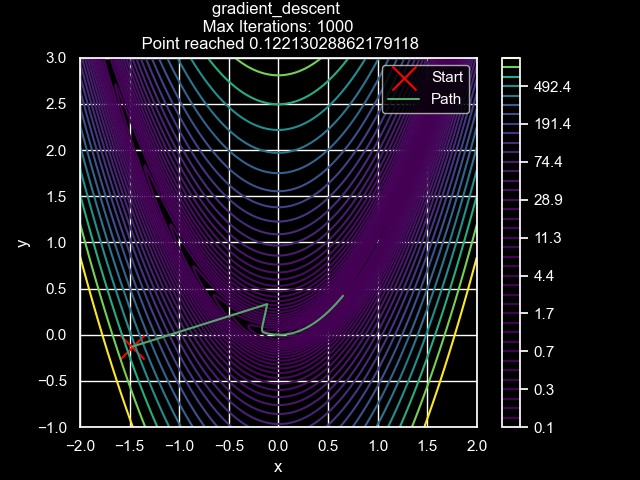
\includegraphics{images/gradient_descent.png}
\caption{Gradient Descent}
\end{figure}

Gradient descent is a baseline here in 1000 generations it minimized the objective function, but did not reach the minima.

\begin{figure}
\centering
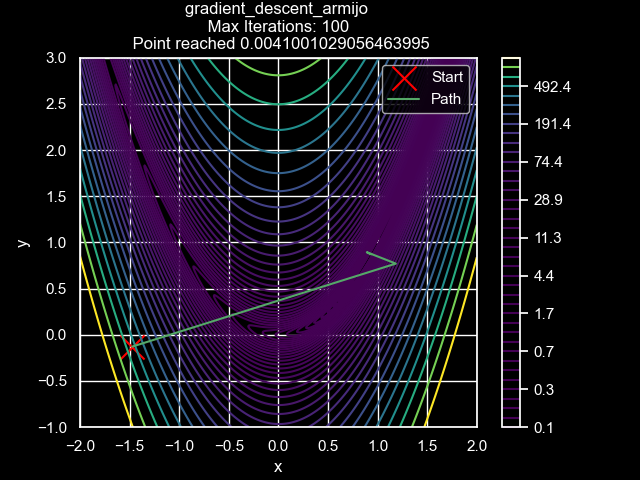
\includegraphics{images/gradient_descent_armijo.png}
\caption{Gradient Descent Armijo}
\end{figure}

Backtracking was able to go further than vanilla gradient descent in fewer iterations adjusting the learning rate until a progress condition as met.

\subsection{Gradient Descent with Momentum}\label{gradient-descent-with-momentum}

\begin{figure}
\centering
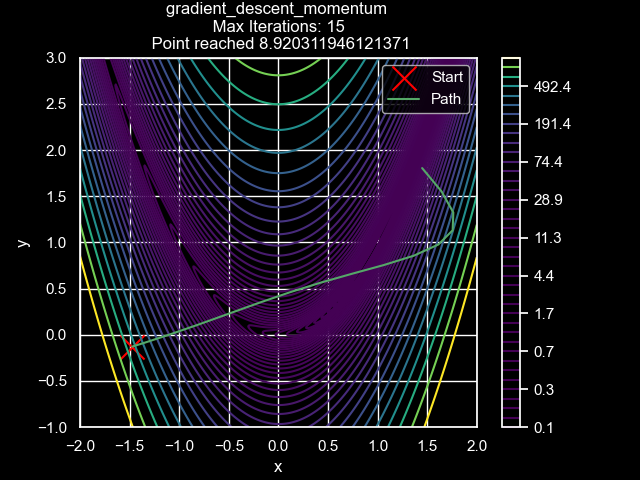
\includegraphics{images/gradient_descent_momentum.png}
\caption{Gradient Descent Momentum}
\end{figure}

Momentum is shown to use very few iterations compared to gradient descent with and without backtracking, but has a tendency to overshoot the minima as it considers previous parameter values to accelerate optimization.

\subsection{Gradient Descent with Nesterov Acceleration}\label{gradient-descent-with-nesterov-acceleration}

\begin{figure}
\centering
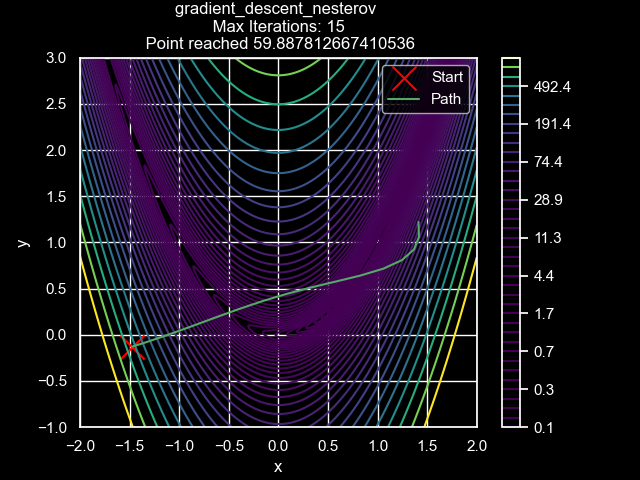
\includegraphics{images/gradient_descent_nesterov.png}
\caption{Gradient Descent Nesterov}
\end{figure}

Nesterov Acceleration is more natural and does not tend to shoot the minimum while taking into consideration previous parameters and providing an accelerated convergence rate.

\subsection{Nesterov With Restart}\label{nesterov-with-restart}

\begin{figure}
\centering
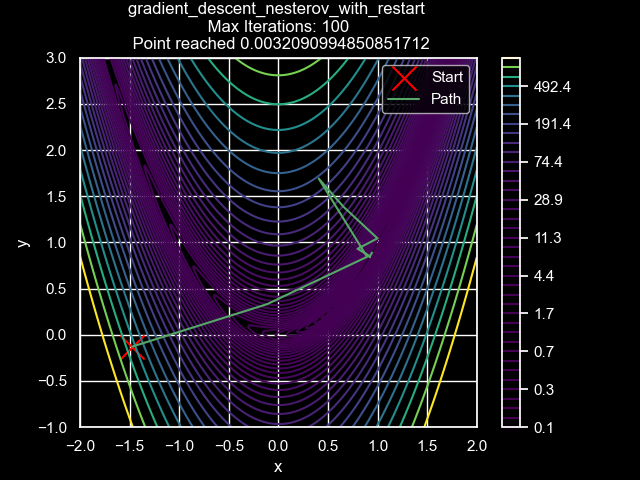
\includegraphics{images/gradient_descent_nesterov_with_restart.png}
\caption{Gradient Descent Nesterov With Restart}
\end{figure}

Restarts are used in Nesterov acceleration ``course correct'' the optimization path. This gives similar results to gradient descent with backtracking in fewer iterations.

\subsection{Newton's Method}\label{newtons-method}

\begin{figure}
\centering
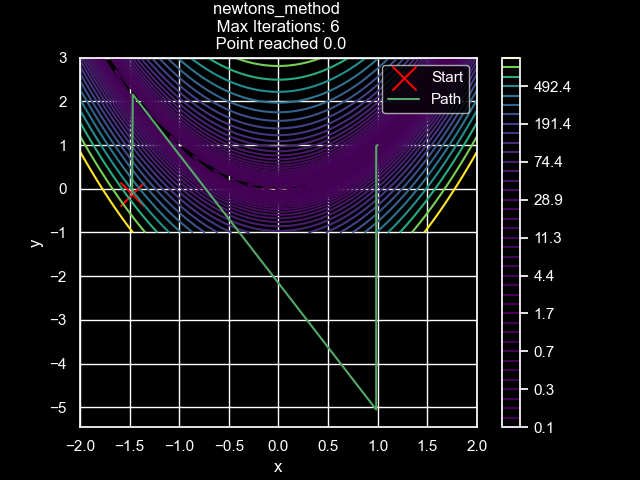
\includegraphics{images/newtons_method.png}
\caption{Newton's Method}
\end{figure}

Newton's method chooses the step size by using the Hessian of the objective function. It is very iteration efficient on this function and reaches the minimum in just six iterations However, the Hessian is expensive to calculate. The part here is a bit erratic to deal with this with damp the Newton update.

\subsection{Damped Newton's Method}\label{damped-newtons-method}

\begin{figure}
\centering
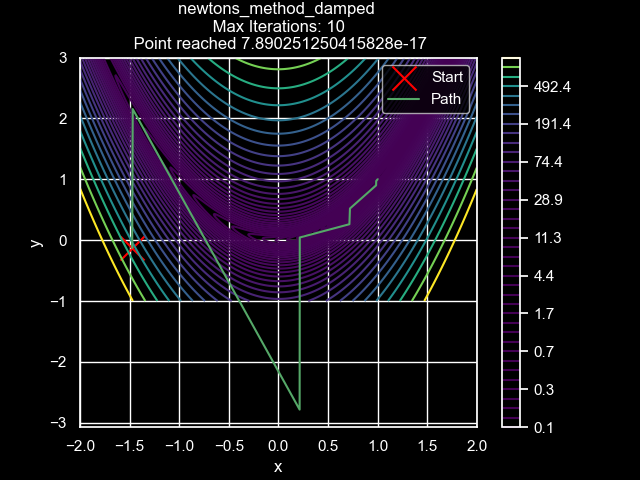
\includegraphics{images/newtons_method_damped.png}
\caption{Newton's Method Damped}
\end{figure}

Damping the Newton update with even 0.999 \((0.999 \times \text{the original update})\) helps a lot in making the optimization more stable. But here it took more iterations to converge.

\subsection{Coordinate Descent}\label{coordinate-descent}

\begin{figure}
\centering
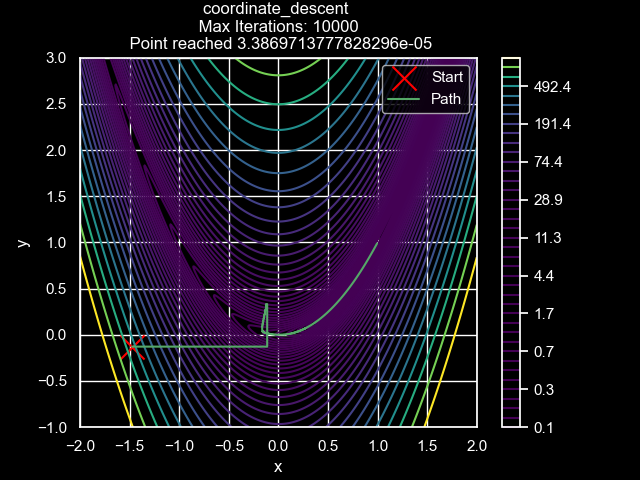
\includegraphics{images/coordinate_descent.png}
\caption{Coordinate Descent}
\end{figure}

Coordinate descent optimizes on one variable at a time, and this can be clearly seen by the nature of the optimization path. In this case, coordinate descent, took quite a few iterations to reach the minima.

\section{Connvolutional Neural Networks}\label{connvolutional-neural-networks}

\subsection{Basics}\label{basics}

Basic neural networks take and perform a linear transformation followed by a non-linear function.

\[
z = h(Wx + b)\\
\text{For single hidden layer network with } W \text{ being a learnable matrix and } b \text{ a learnable vector.}
\]

These layers can be stacked together to for a larger network which consists of ``dense'' or fully connected linear layers that pass through a non-linear ``activation'' function before moving onto the next layer.

\[
y = h_3(W_3 \cdot (h_2(W_2 \cdot h_1(W_1 x + b+1) + b_2)) + b)\\
\text{This network has 3 hidden layers.}
\]

As the data comes in it is mapped to space where it is more linearly separable. The mapping is learned from the data using backpropagation and variations of gradient descent.

\textbf{Need for convolutional neural networks?}

The issue with dense networks is the number of parameters and sizes of inputs quickly gets out of hand. A tiny \(100 \times 100\) gray image has \(10,000\) parameters. Assuming the output is predicting what number a picture of a digit is, the size of the output layer is 10 (0 - 9 digits). This yields a network with at least \(10,000 \times 10 = 100, 000\) parameters. This is huge for an impractically small image size and modern networks have output sizes of in the tens if not hundreds of thousands.

The second issue is if you feed a picture into a dense neural network, you would have to flatten the image's \(n\)-dimensional array. So a \(100 \times 100\) image matrix becomes a \(10,000\) sized vector. This leads to a total loss of structure in an image which means we completely ignore the spatial locality that helps us identify what a picture contains. For example, a picture of an apple is likely to have a specific curvature.

We need a way to reduce the size of the input leading to a reduced set of parameters. And we need a way to learn spacial localities from data. That is where convolutional neural networks come into play.

\subsection{Convolutions}\label{convolutions}

Assume discrete data with a height and width, like a gray image. A convolution can be mathematically expressed as:

\[
(I * K)(i, j) = \sum_{m=-k}^{k} \sum_{n=-k}^{k} I(i-m, j-n) \cdot K(m, n)\\
\text{Where } I \text{ is the image.}\\
\text{And } K \text{ is a relatively tiny matrix called a kernel or a filter.}
\]

Intuitively, this operation slides a tiny matrix over the image and computes a dot product at each stage. This changes the image and highlights things tat resemble the kernel. You can pass the convolved image through a non linear function \(h\) to produce more complex patterns.

Convolutions help capture spacial localities from data. This is especially useful in images to learn underlying patterns. But, convolutions are helpful in all kinds of data gain meaning from ``what is around'' features in the data. For example, speech data, flow fields and signals. This notion is useful in neural networks and can be found in convolutional layers.

\subsection{Convolutional Layers}\label{convolutional-layers}

Convolutional layers allow neural networks to learn spatial localities in data for example the flow of fluid or features in an image. Convolutional filters are randomly initialized before training and learn to highlight certain teaches from the data. They can drastically reduce the number of parameters needed in a network.

\begin{figure}
\centering
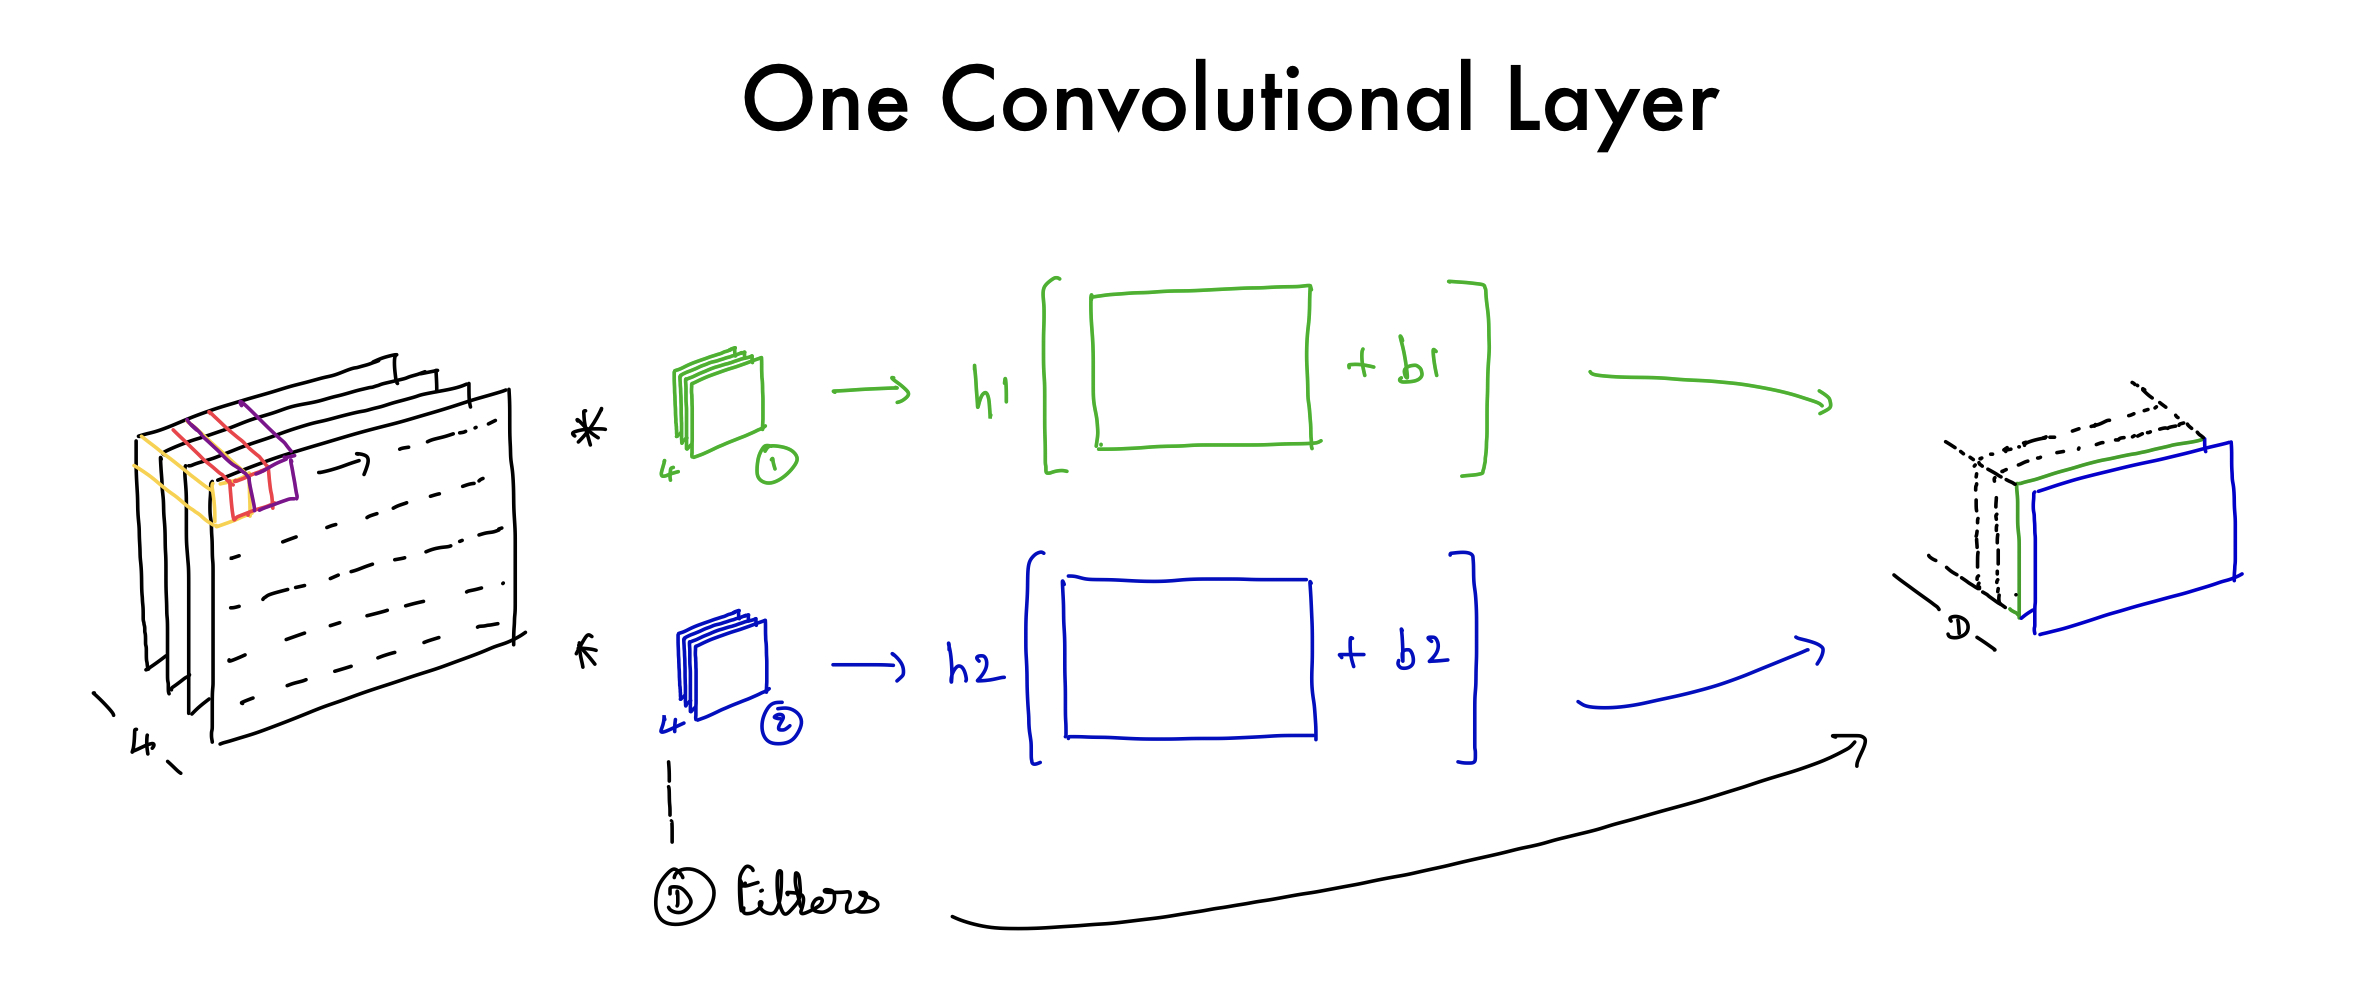
\includegraphics{images/IMG_0008.jpg}
\caption{One Convolutional Layer}
\end{figure}

Filters are typically the same depth as the impact that they receive once the filter has been convolved over the image. a bias is added, and the whole thing is passed through a non-linearity assuming you use D filters you will get an output of depth D for that particular layer.

In the above picture, the large image with depth 4 it convolved with two small filters also of depth 4. Then bias is added to each output and fed through a non-linear function. The output will be of depth 2.

The size of an image after a convolution of course depends on the stride (how many pixels you skip while you slide over) and the padding (how you deal with the boundary).

\subsection{Pooling layers}\label{pooling-layers}

\begin{figure}
\centering
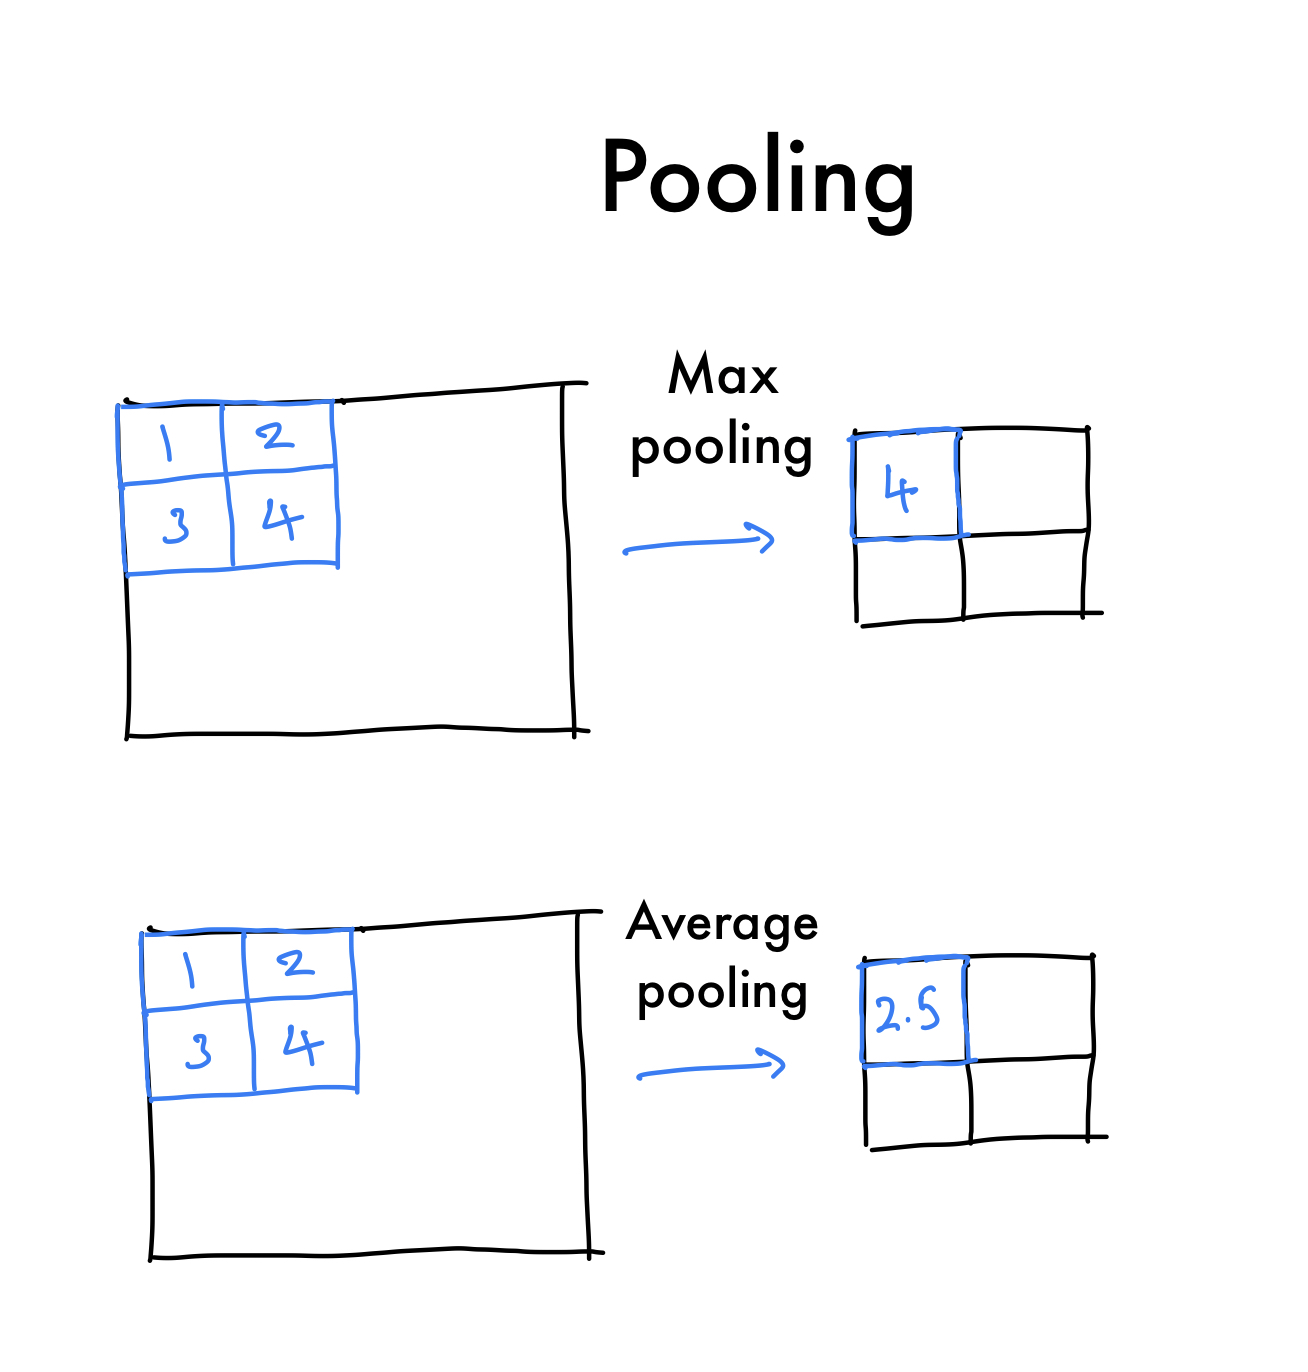
\includegraphics[width=0.5\textwidth,height=0.5\textheight]{images/pooling.jpeg}
\caption{Pooling Layers}
\end{figure}

Pooling layers are \textbf{do not include learnable parameters}. They are used to reduce the height and width of your data as well as build invariances from data that help in generalization and making the model more robust. There are two types of pooling - \textbf{max} pooling and \textbf{average} pooling.

Pooling is done using a \(k \times k\) filter that is slid over the image and either the \textbf{maximum} or \textbf{average} value of numbers in the kernel is kept thereby reducing the size of the data passing through the pooling layer. These layers are typically placed after convolutional layers.

\subsection{Example}\label{example}

Below is an example convolutional neural network with two convolutional layers and two linear layers:

\begin{figure}
\centering
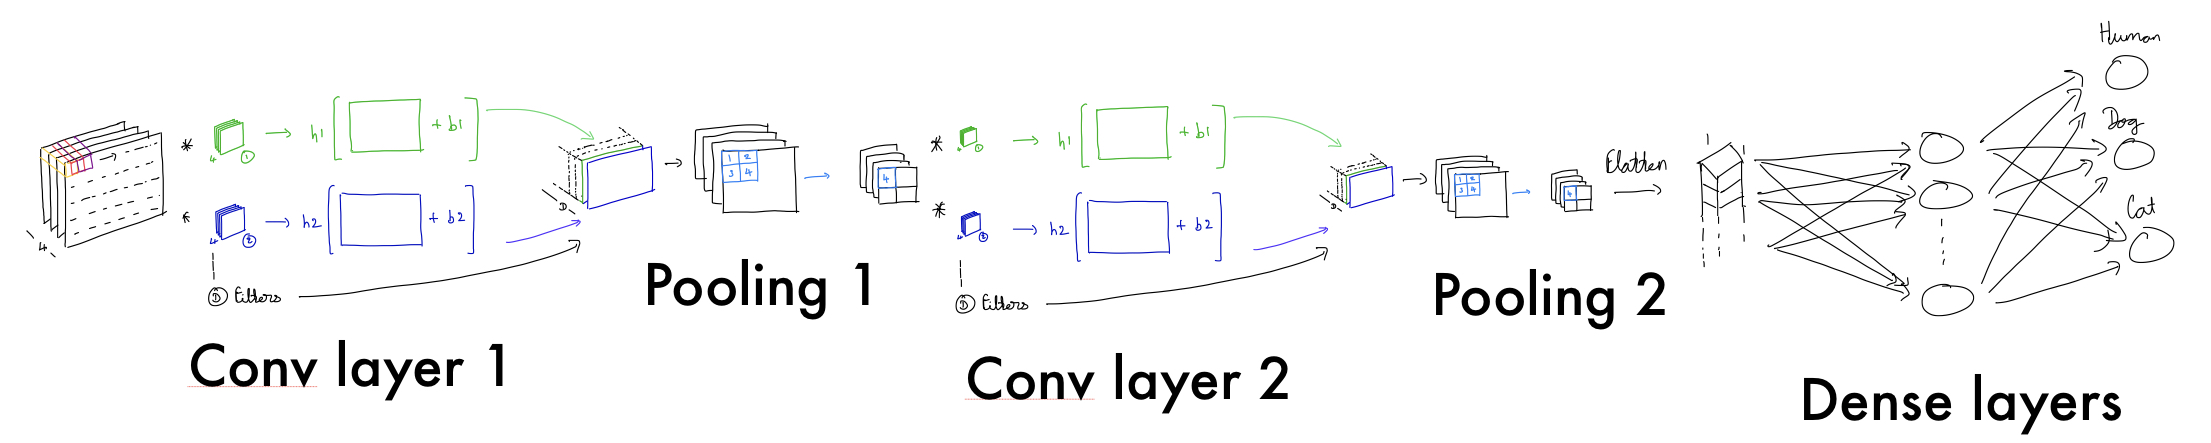
\includegraphics{images/cnnexample.jpeg}
\caption{Example}
\end{figure}

\[
I_1(c_1, i, j) = h_{conv_1}\left[\sum_{c=1}^{3} \sum_{m=-k_1}^{k_1} \sum_{n=-k_1}^{k_1} I(c, i-m, j-n) \cdot K_1(c_1, c, m, n) + b_{conv_1}\right] \\\\
\quad \\
P_1(c_1, i, j) = \max_{m,n \in \{0, \ldots, p_1-1\}} I_1(c_1, i \cdot p_1 + m, j \cdot p_1 + n) \\\\
\quad \\
I_2(c_2, i, j) = h_{conv_2}\left[\sum_{c_1=1}^{C_1} \sum_{m=-k_2}^{k_2} \sum_{n=-k_2}^{k_2} P_1(c_1, i-m, j-n) \cdot K_2(c_2, c_1, m, n)+ b_{conv_2}\right] \\\\
\quad \\
P_2(c_2, i, j) = \max_{m,n \in \{0, \ldots, p_2-1\}} I_2(c_2, i \cdot p_2 + m, j \cdot p_2 + n) \\\\
\quad \\
f = \text{flatten}(P_2) \\\\
\quad \\
z_1 = h_1(W_1 f + b_1) \\\\
\quad \\
Y = h_2(W_2 z_1 + b_2) \\\\
\]

\subsection{Conclusion}\label{conclusion}

Convolutional layers allow us to extract features from our input in hierarchical way. Let us see we are training a CNN predict if an image is a human, dog or cat using say 3 convolutional layers followed by some fully connected layers where the output is three neurons.

The first convolutional layer might have a certain set of filters that detect edges and boundaries. The second convolutional might have a set of filters that detect eyes, noses, ears and hair. And the third set of filters in a convolutional layers might detect limbs and appendages. At each stage some of these filters might only light up if they see, for example, see a human hand but not light up when they see a dogs paw. That condensed information is the flattened and passed through fully connected layers to finally predict what the image is.

For more information see \href{https://yosinski.com/media/papers/Yosinski__2015__ICML_DL__Understanding_Neural_Networks_Through_Deep_Visualization__.pdf}{this} paper.

\textbf{Fully Convolutional U-NET Type architecture}

\begin{figure}
\centering
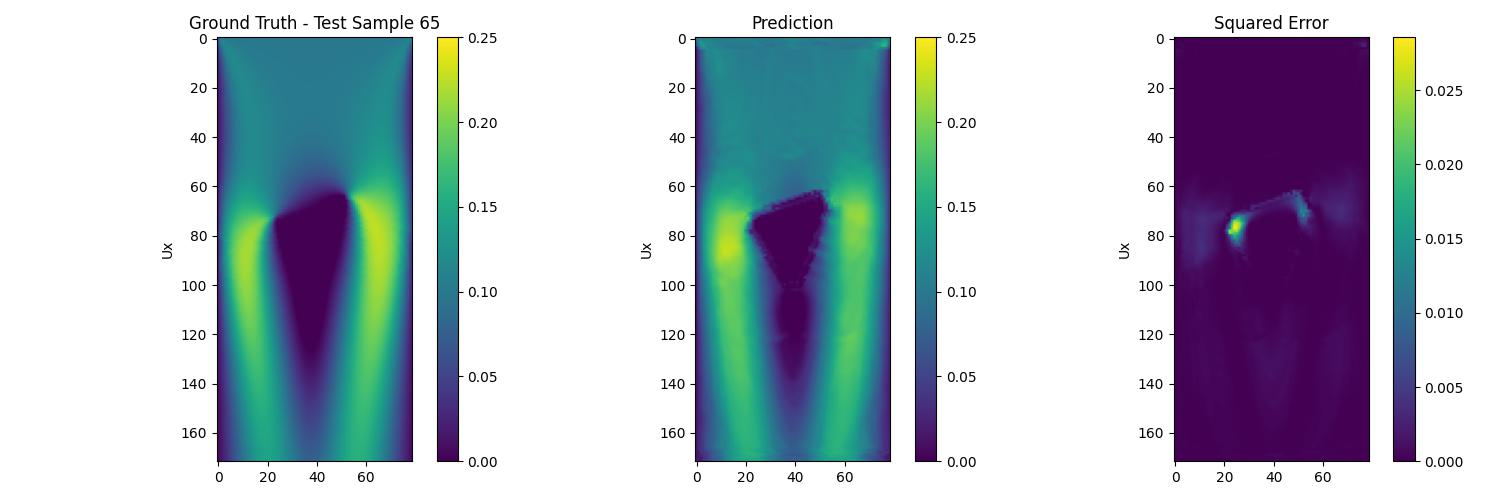
\includegraphics{CNN_Fluids/figures/testset.jpg}
\caption{Flow Approximation}
\end{figure}

This is a prediction (from a test set) using a simplified UNET based fully convolutional neural network.

The network takes in data from distance functions from the object and a flow region channel where each number represents information of the flow - 0 for the obstacle, 1 for the free flow region, 2 for the upper/bottom no-slip wall condition, 3 for the constant velocity inlet condition, and 4 for the zero-gradient velocity outlet condition.

\section{Recurrent Neural Networks}\label{recurrent-neural-networks}

\subsection{Background}\label{background}

The problem with fixed size neural networks, even with convolutional layers, is that thy cannot handle input a variable input size like a sentence with \(k\) words. You could pass in one word at a time but each input will be treated independently. It is the same with images, you could pass in 10 frames of a video in a convolutional networks one after the other but there wont be any relation to the temporal component of the video. Each frame will be treated as its own separate image. This is because regular neural networks don't take into account past inputs in a sequence.

\[
y = h(Wx+b)
\]

\subsection{Introduction}\label{introduction-1}

To handle sequential data, we can define a neural network that updates it's weights based on previous data from a sequence.

\[
h_t = f_1(W_{h} h_{t-1} + W_{x} x_{t} + b_h) \\
y = f_2(W_{y} h_{t} + b_y)
\]

Here, \(W_{x} x_{t}\) is the standard matrix multiply used in regular neural networks. \(W_hh_{t-1}\) relates the inputs in a sequence together. \(W_{h}, W_{x}, W_{h}, b_h, b_y\) are shared across the temporal time component \(t\). For each time-step \(t\), a new \(h\) and \(y\) is calculated. \(x_0\) is usually initialized to the \(0\) vector or randomly. The intuition here is that the weights are updated taking into account the whole sequence.

\subsection{Types of RNN's}\label{types-of-rnns}

RNN's can be represented as -

\begin{figure}
\centering
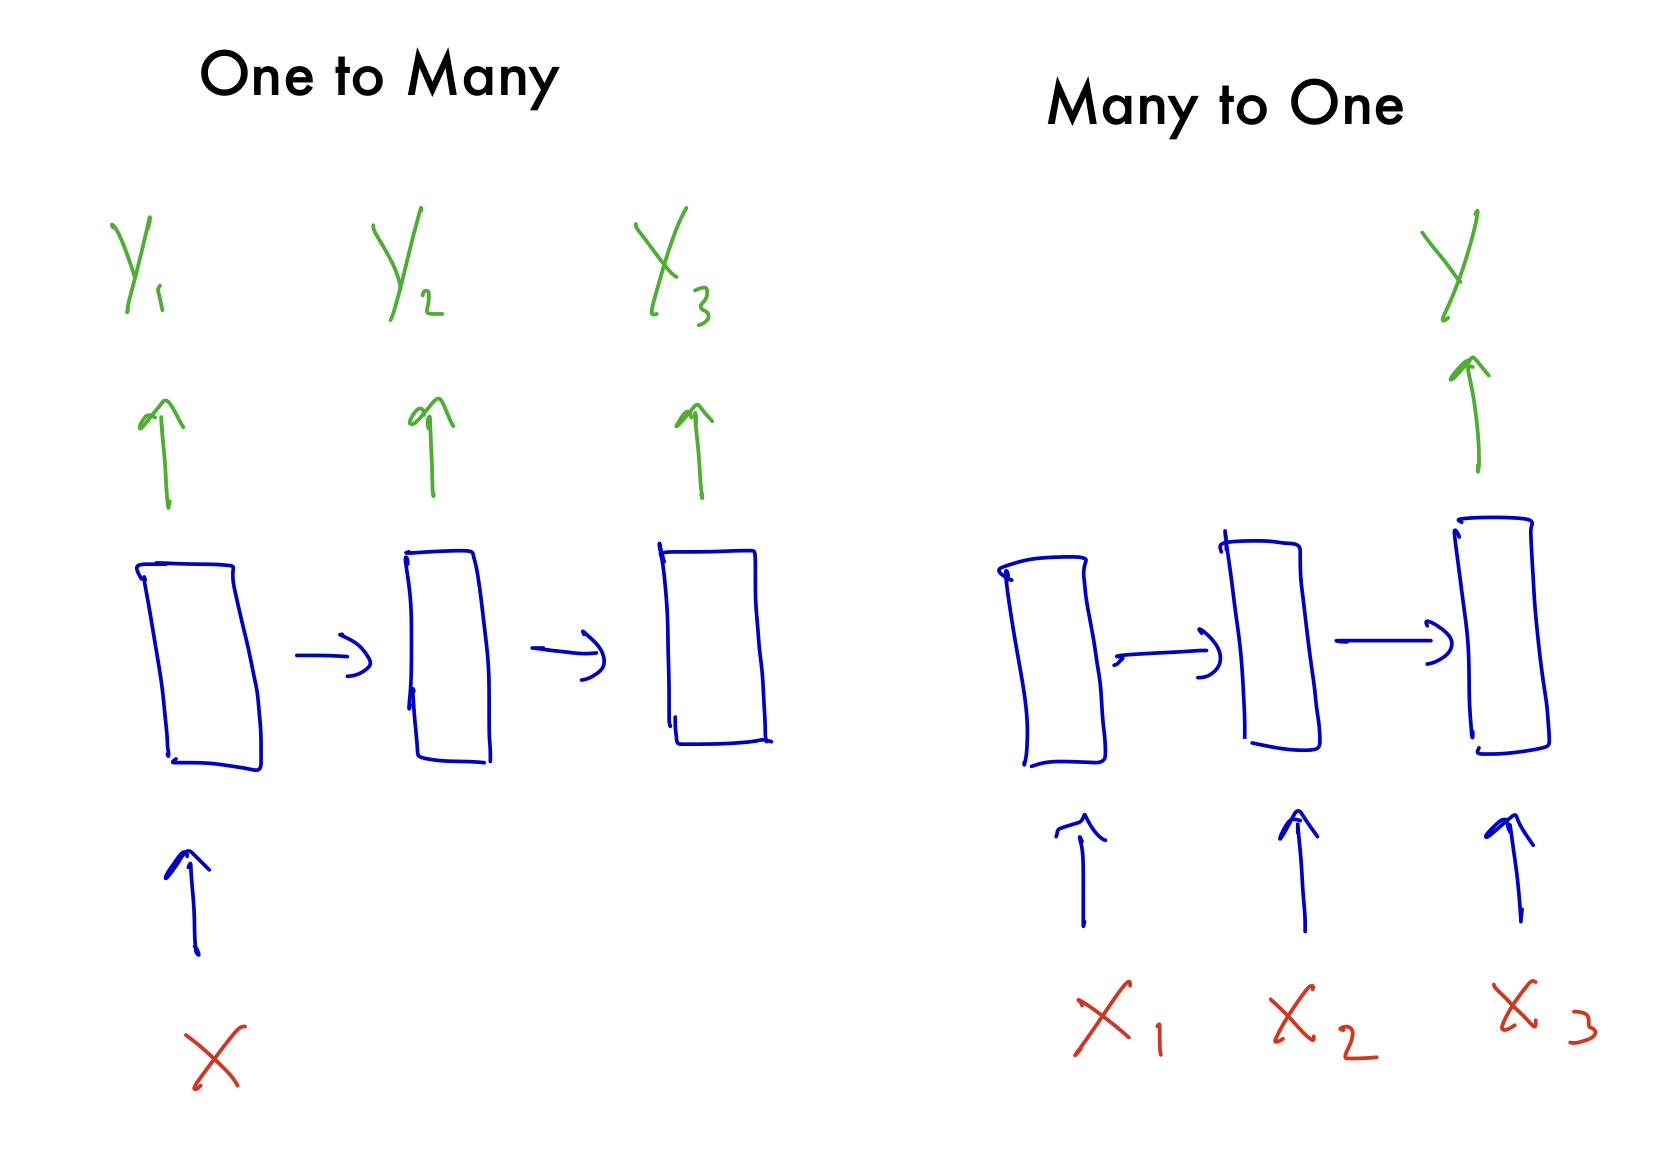
\includegraphics{images/IMG_0012.jpg}
\caption{RNN}
\end{figure}

The cyclic arrow represents the network updating at a time interval \(t\). This can be used to represent any recurrent neural network but we can be more concrete. There a some common arrangements that can be useful in different situations.

\subsubsection{One to many}\label{one-to-many}

These networks take in one input (a sequence of size 1), and produce of sequence of any size. For example, the input may be an image of fixed size and the output is a caption sequence of any size.

\subsubsection{Many to one}\label{many-to-one}

These networks take in an input sequence of variable size and give us one output. For example, the input may be a sentence sequence of variable size and the output is the sentiment of the sentence.

\begin{figure}
\centering
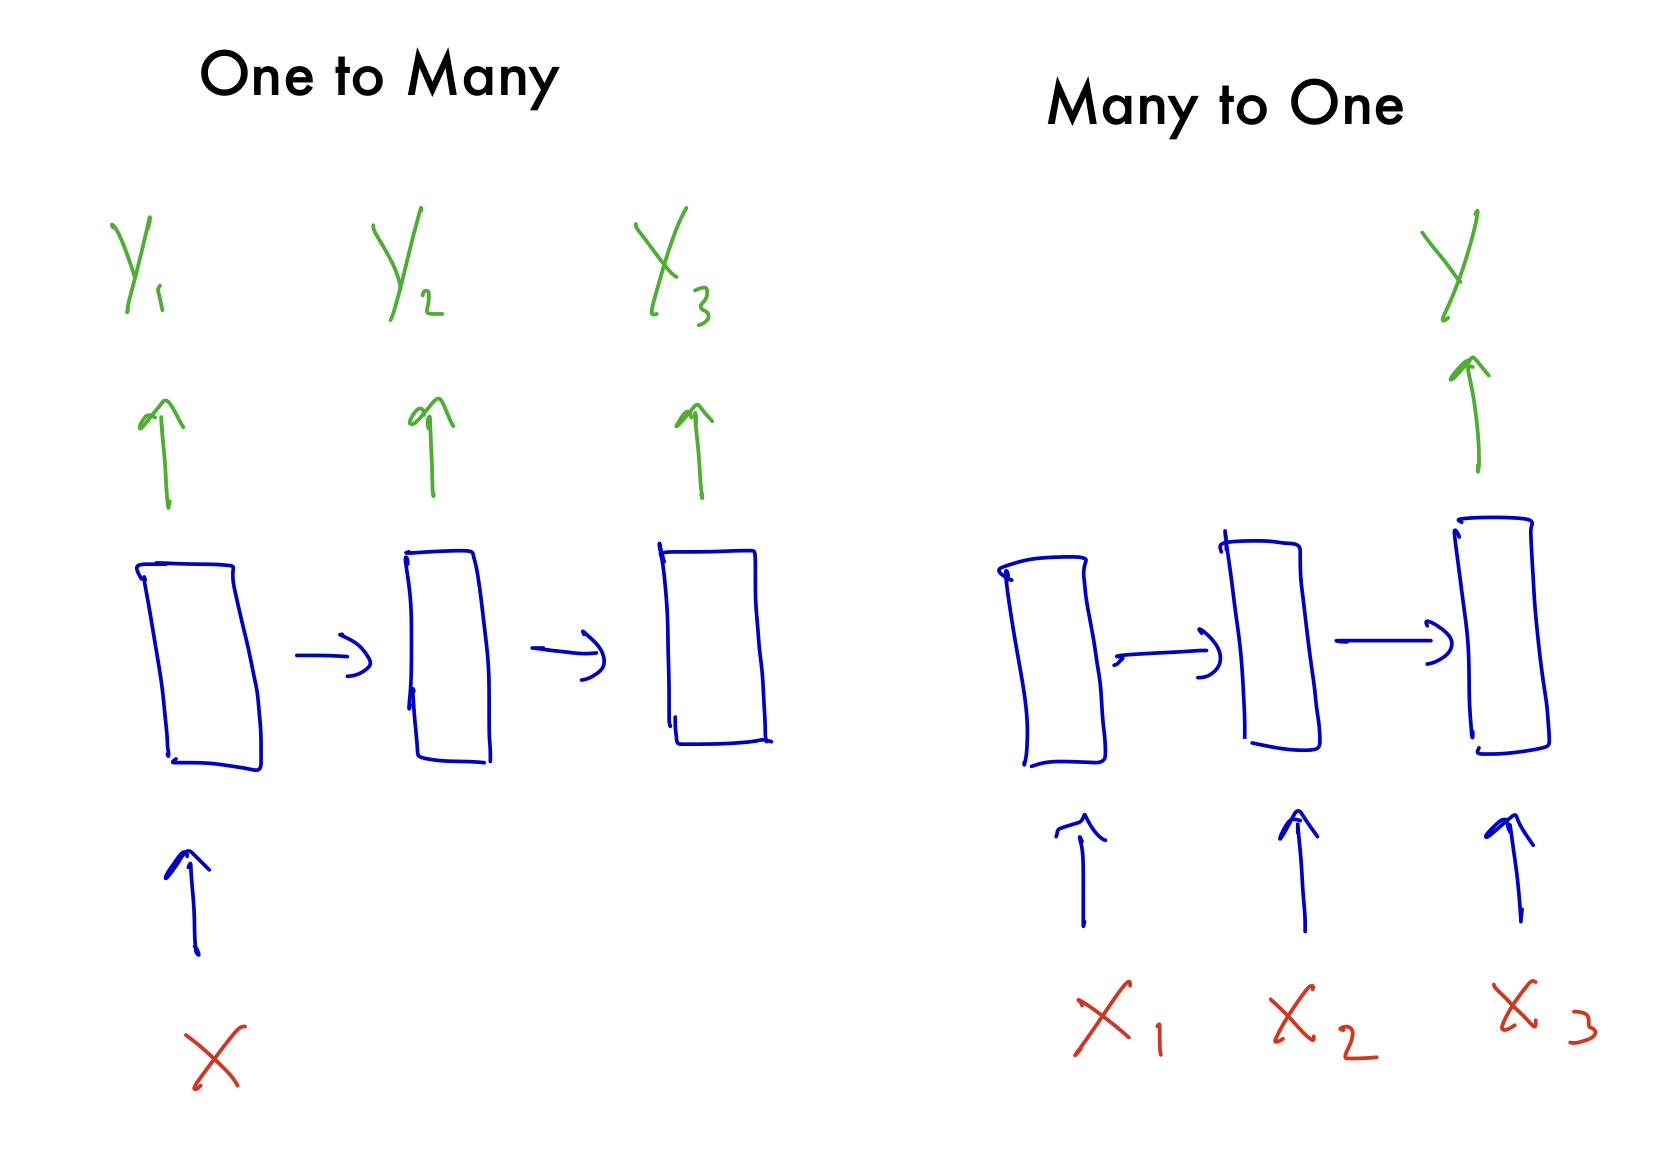
\includegraphics{images/IMG_0012.jpg}
\caption{One to Many \& Many to One}
\end{figure}

\subsubsection{Many to Many}\label{many-to-many}

Here, the input and output have a variable sequence length. For example, using deep learning to translate from one language to another. We could also have a video with multiple frame and we can do segmentation or classification or segmentation over frames of the image.

\begin{figure}
\centering
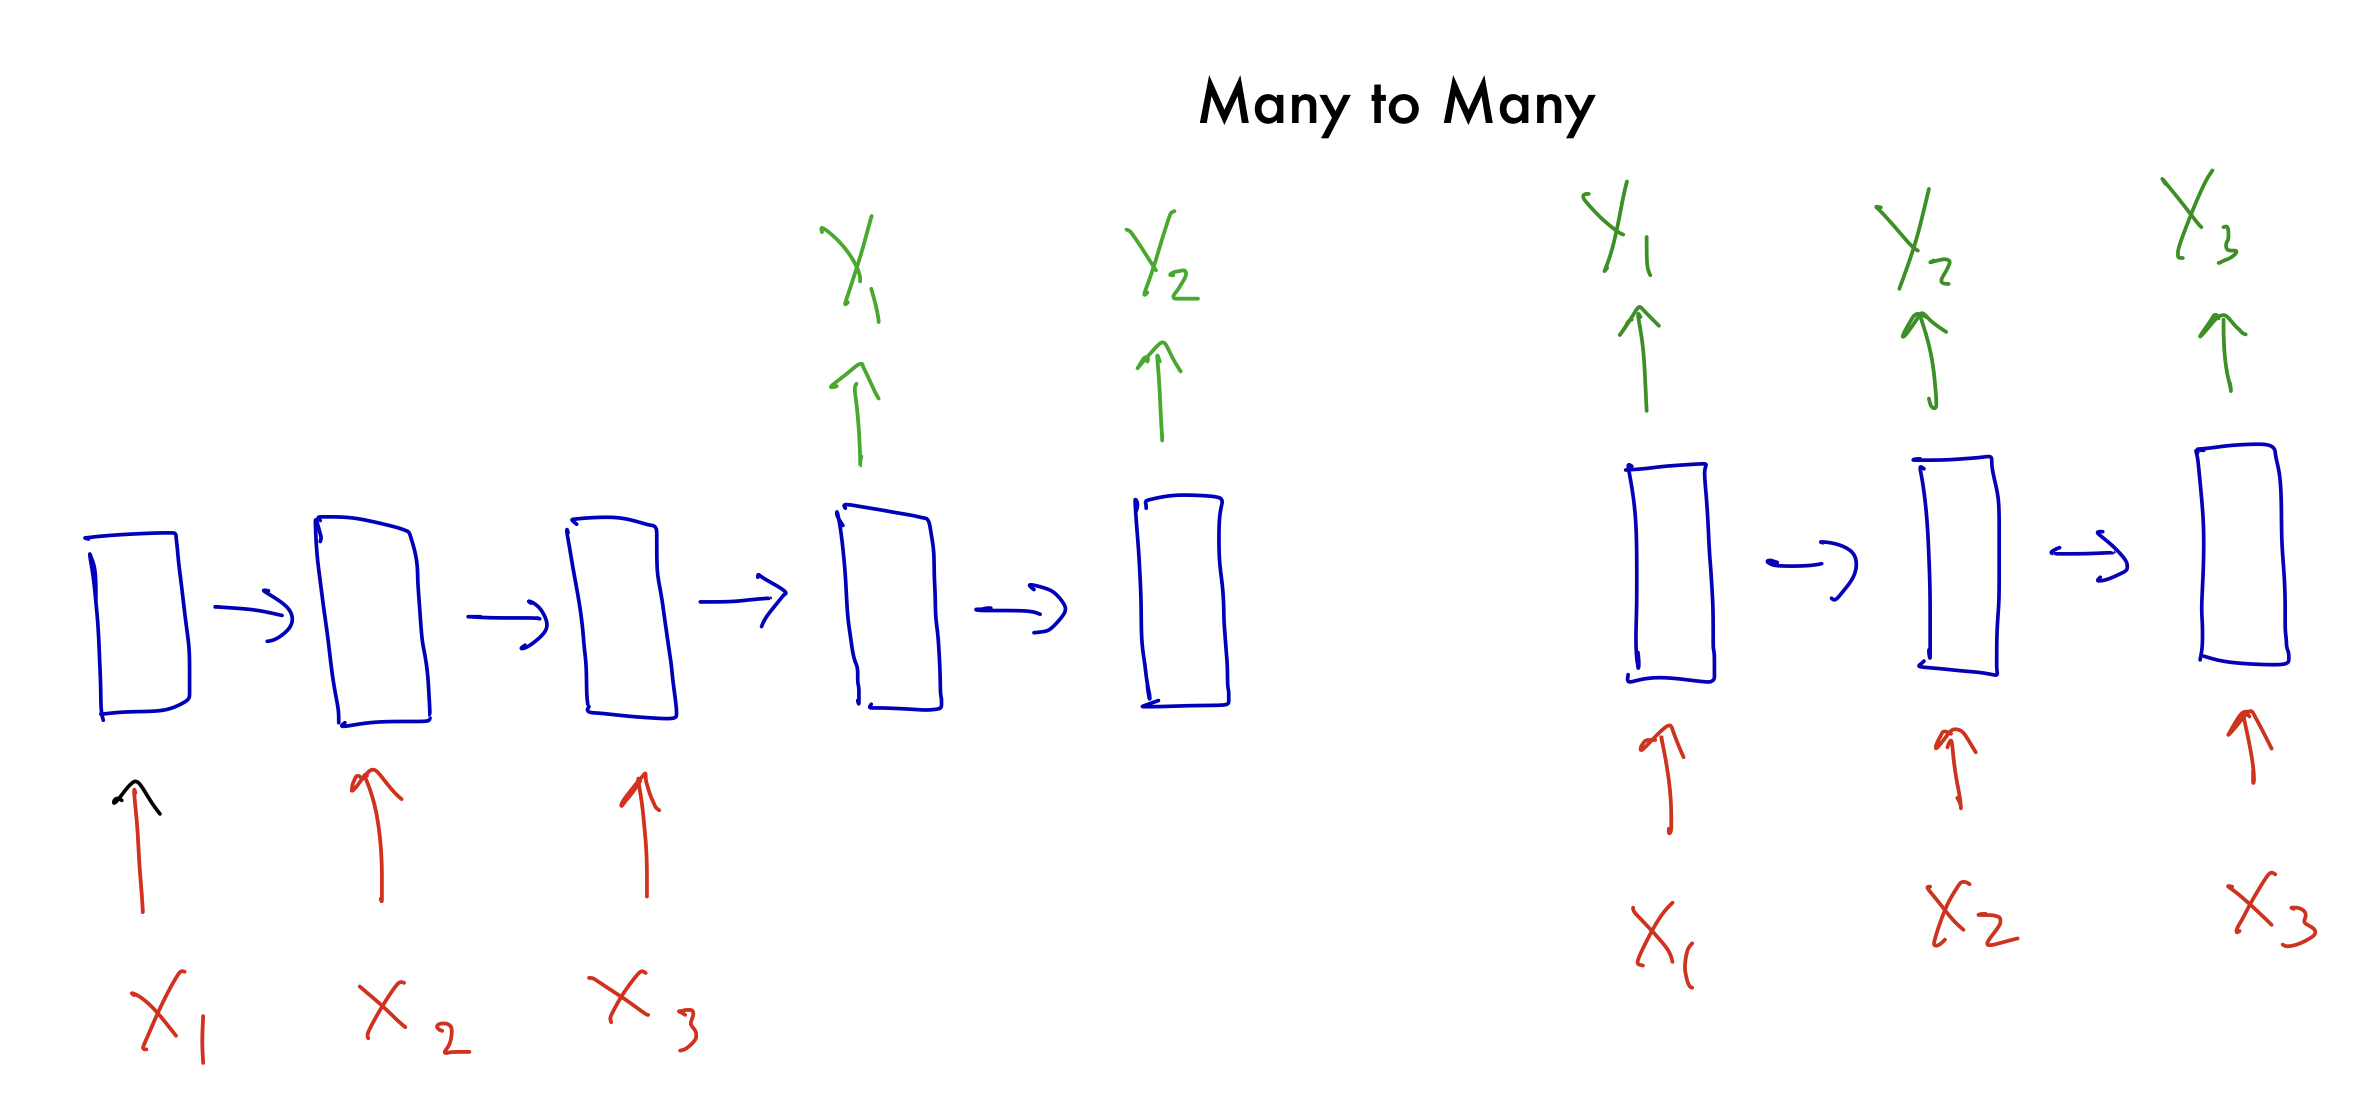
\includegraphics{images/IMG_0013.jpg}
\caption{One to Many \& Many to One}
\end{figure}

\subsection{Problems with (Basic) RNN's}\label{problems-with-basic-rnns}

We do backpropagation on the ``unrolled'' RNN. But when we do this we run into problems as the gradient passes through this unrolled network. More concretely:

Let us consider 3 iterations of \(h_t\)
\[
h1 = g(W_hh0 + W_xx1) \\
h2 = g(W_hh1 + W_xx2) \\
h3 = g(W_hh2 + W_xx3) \\
\]
Let \(L\) be a loss function

\[
\frac{\partial L_{}}{\partial W_{h}} =
\frac{\partial L_{}}{\partial h_{3}} \frac{\partial h_{3}}{\partial W_{h}} +
\frac{\partial L_{}}{\partial h_{3}} \frac{\partial h_{3}}{\partial h_{2}} \frac{\partial h_{2}}{\partial W_{h}} +
\frac{\partial L_{}}{\partial h_{3}} \frac{\partial h_{3}}{\partial h_{2}} \frac{\partial h_{2}}{\partial h_{1}} \frac{\partial h_{1}}{\partial W_{h}}\\
\phantom{1}\\
\frac{\partial L}{\partial W_{h}} = \frac{1}{n} \sum_{t=1}^{n} \frac{\partial L_{t}}{\partial h_{t}} \prod_{j=i+1}^t \frac{\partial h_{j}}{\partial h_{j-1}} \frac{\partial h_{i}}{\partial W_{h}}
\]

If the gradients are consistently more than 1, the gradient is multiplied \(t\) times and explodes resulting in a overflow. If the gradients are consistently less than 1, the gradient is multiplied \(t\) times and vanishes resulting in a underflow.

\end{document}
